%!TEX program = xelatex

\documentclass[openany]{progbookcn}

\usepackage{wrapfig}
\usepackage{enumerate}
\usepackage{amsmath,mathrsfs,amsfonts}
\usepackage{tabularx}
\usepackage{booktabs}
\usepackage{colortbl}
\usepackage{multirow,makecell}
\usepackage{multicol}
\usepackage{ulem} % \uline
\usepackage{listings}
\usepackage{tikz}
\usepackage{tcolorbox}
\usepackage{fontawesome}
\usepackage[open,openlevel=0,atend]{bookmark}
\usepackage{graphicx}
\usepackage{float} 
\usepackage{subfigure}
\usepackage{enumitem}
\usepackage{ctex}

% 用来设置附录中代码的样式

\lstset{
    basicstyle          =   \sffamily,          % 基本代码风格
    keywordstyle        =   \bfseries,          % 关键字风格
    commentstyle        =   \rmfamily\itshape,  % 注释的风格,斜体
    stringstyle         =   \ttfamily,  % 字符串风格
    flexiblecolumns,                % 别问为什么,加上这个
    numbers             =   left,   % 行号的位置在左边
    showspaces          =   false,  % 是否显示空格,显示了有点乱,所以不现实了
    numberstyle         =   \zihao{-5}\ttfamily,    % 行号的样式,小五号,tt等宽字体
    showstringspaces    =   false,
    captionpos          =   t,      % 这段代码的名字所呈现的位置,t指的是top上面
    frame               =   lrtb,   % 显示边框
}

\lstdefinestyle{Python}{
    language        =   Python, % 语言选Python
    basicstyle      =   \zihao{-5}\ttfamily,
    numberstyle     =   \zihao{-5}\ttfamily,
    keywordstyle    =   \color{blue},
    keywordstyle    =   [2] \color{teal},
    stringstyle     =   \color{magenta},
    commentstyle    =   \color{red}\ttfamily,%注释
    breaklines      =   true,   % 自动换行,建议不要写太长的行
    columns         =   fixed,  % 如果不加这一句,字间距就不固定,很丑,必须加
    basewidth       =   0.5em,
}

\setenumerate[1]{itemsep=0pt,partopsep=0pt,parsep=\parskip,topsep=5pt}
\setitemize[1]{itemsep=-1pt,partopsep=0pt,parsep=\parskip,topsep=0pt,itemindent=5pt}
\setdescription{itemsep=0pt,partopsep=0pt,parsep=\parskip,topsep=5pt}
%=========英文字体
\usepackage[osf]{libertinus-otf} 
\usepackage{imakeidx}
\makeindex[%
  intoc=true,
  columns=2,
  columnsep=1cm,
  columnseprule=true
]


\begin{document}

%% title page
\begin{titlepage}
  \vspace*{25ex}

  \hspace{0.05\textwidth}\begin{minipage}{.9\textwidth}
    \flushright

    %%中文书名
    {\zihao{1}\textbf{数学建模竞赛学习笔记}}

    \rule{\linewidth}{.5pt}

    \vspace{2ex}

    %% 副标题
    {\zihao{2}\textsf{从理论到实战}} \\

    \vspace{20ex}

    %% 作者
    {\zihao{4}\textit{谷文军}}
  \end{minipage}

  \vfill

  \centering
  {\zihao{4}镇江 ~$\bullet$ ~ZHENJIANG}
\end{titlepage}
\thispagestyle{empty}


\frontmatter


\chapter{序}

数学建模。

\chapter{前言}


%% 目录
\clearpage
{
  \hypersetup{hidelinks}
  \tableofcontents
}


\mainmatter

\part{数学建模基础}


\chapter{绪论}



\section{绪论}



\chapter{数学建模的思想与方法}

\section{建模步骤}
8步建模法
\subsection{问题提出}
\begin{itemize}
\item 了解实际问题的背景(属于哪一个领域)
\item 明确数学建模的目的(解决什么问题)
\end{itemize}

\subsection{量的分析}
\begin{itemize}
\item 收集数学建模的必要信息(相关数据和参考资料)
\item 分析研究对象的主要特征(内在机理或输入输出)
\end{itemize}

\subsection{模型假设}
根据所研究的对象特征及建模目的,抓住问题本质,忽略次要因素,对问题做出合理的简化假设(基本符合实际情况,能够用数学语言描述问题)。
\subsection{模型建立}
根据假设,用数学语言、符号描述出研究对象的内在规律,并建立包含常量、变量等的数学模型,可以是函数表达公式、数学方程、数据表格、算法或图形甚至是一段文字描述。
\subsection{模型求解}
采用各种计算方法对所建立的数学模型进行求解,可能是求函数的极值、求方程的解、算法或图形的实现等。
\subsection{模型分析}
\begin{itemize}
\item 对求解结果进行数学上的分析
\item 包括结果的误差分析(误差是否在允许范围内)
\item 统计分析(结果是否符合特定的统计规律)
\item 模型对数据的灵敏度分析(模型的结果是否会因数据的微小变化而发生大的变化)
\item 对假设的鲁棒性分析(robustness)(模型的结果是否对某一假设非常依赖?)等
\end{itemize}
\subsection{模型检验}
\begin{itemize}
\item 将求解结果和分析结果翻译回到实际问题之中,与实际现象、实际数据进行比较,检验是否与实际吻合。
\item 如果吻合较好,则模型及其结果可以应用于实际。如果吻合不好,则需要对模型进行修正。
\item 此时问题常常出现在模型假设上(假设是否合理,是否忽略了重要因素而保留了次要因素),所以应对模型假设进行修正或补充,然后重新建模。 

\end{itemize}
\subsection{模型应用}
当模型经过检验已成为一个具有合理性和实用性的模型后,即可以用来解决实际问题。
\section{建模方法}

\subsection{机理分析法}
在对研究对象内部机理分析的基础上,利用建模假设所给出的建模信息或前提条件及相关领域知识、相应的数学工具来构造模型。
\subsection{系统识别建模法}
对系统内部机理不清楚的情况下,利用建模假设或对系统进行实际测试所得到的数据信息,再运用数学方法确定模型形式,借助于概率论和数理统计来辨识参数,构造模型。
\subsection{仿真建模法}
利用各种仿真方法建模。
\subsection{相似类比建模法}
借助于相似原理和事物之间的类比关系进行建模的方法,即根据不同对象之间的某些相似性,借用移植领域的数学模型构造数学模型的方法。


\section{分类与特点}
\subsection{数学建模的分类}
\begin{itemize}
\item {按建模的数学方法划分}\\
初等模型、数学规划模型、微分方程模型、差分方程模型、概率统计模型、图论模型、模糊模型和灰色模型等。
\item {按建模中变量特点划分}\\
确定性模型与随机性模型、静态模型与动态模型、线性模型与非线性模型、离散模型与连续模型等
\item {按应用领域划分}\\
人口模型、交通模型、环境模型、规划模型、生态模型、资源模型等
\item {按建模目的划分}
描述模型、预测模型、优化模型、决策模型、控制模型等
\item {按照对问题的了解程度划分}\\
白箱模型、黑箱模型、灰箱模型

\end{itemize}

\subsection{数学建模的特点}
\begin{itemize}
\item{逼真性和可行性}\\
模型越逼真就越复杂,应用起来费用就越高,常与取得的效益不成正比,所以需要对逼真性与可行性进行折中
\item{渐进性}\\
数学模型通常不会是一次就成功的,往往需要反复修正,逐渐完善
\item{健壮性}\\
对于已经建好的数学模型,当观测数据有微小的改变或者模型结构及参数发生微小变化时,模型求解的结果也随之发生微小的变化
\item{可移植性}\\
数学模型是现实对对象抽象化的产物,它可能与其他领域或其他事物有共性,常常好多领域不同事物却有几乎相同的数学模型
\item{非预制性}\\
建模时遇到的问题往往事先没有答案,因此必须创新,产生新方法、新概念
\item{条理性}\\
从建模角度出发,人们对现实对象分析应该全面、深入,更具有条理性。即使建模失败,对解决研究实际问题也是有利的
\item{技艺性}\\
建模与其说是一门技术,不如说是一种技艺很强的技巧艺术,建模期间经验、想象力、洞察力、判断力以及直觉灵感起的作用往往比数学知识更大
\item {局限性}\\
由于建模时往往把显示对象简化、近似、假设,因此当模型应用到实际时就必须考虑被忽略的简化因素,于是结论往往是相对的、近似的。另外,由于人类认识能力受科学技术以及数学本身发展水平的限制,至今还有不少实际问题没有建立出有价值实用的数学模型
\end{itemize}

\section{数学建模能力的培养}
\begin{itemize}
\item 数学知识的积累
\item 多看、多学数学建模案例
\item 培养观察能力和用数学解决问题的思想
\item 需要丰富的想象力与敏锐、深刻的洞察力
\item 兴趣是学习的动力,努力培养建模兴趣
\item 与计算机紧密关联,学会使用相关软件
\item 注意团队意识和团结协作
\item 学会类比,做到“由此及彼和由彼及此”,培养发散思维能力
\item 培养自学能力,能快速获取新知识,并能学以致用
\item 从杂乱无章的各种信息中快速挑选收集有用信息,利用图书馆、网络查找相关资料
\end{itemize}

\part{数学建模方法}

\chapter{初等方法建模}
\section{勾股定理与黄金分割率}
\subsection{黄金分割应用于高跟鞋问题}
\noindent\textbf{原理}:人的下肢长占身高的0.618时,满足最佳黄金比例。\\
\textbf{计算黄金分割最简单的方法}:\\
设某人身高为$h$ cm,下肢长$h_1$ cm,选择高跟鞋的鞋跟高度为$x$ cm,则由建模原理得:
\begin{equation}
{{x+h_1}\over{x+h}}=0.618
\end{equation}
解得:
\begin{equation}
x={{0.618h-h_1}\over 0.382}
\end{equation}
\subsection{黄金分割在其他领域的应用}
\noindent \textbf{医学与0.618的联系}
\begin{itemize}
\item 外界环境温度为人体温度的0.618倍时,人会感到最舒适
\item 养生之道:动与静是一个0.618的比例关系,即四分动六分静是人们认为的最佳养生方式
\item 吃饭六七成饱,几乎不生胃病
\end{itemize}
\noindent \textbf{建筑学与0.618的联系}\\
\noindent \textbf{黄金矩形}

\section{九宫图}
\subsection{九宫图问题的提出}
九宫图又称为三阶幻方,出自西汉(公元前206-公元25)学者戴德编纂的《大戴礼》,源自河图洛书。
\begin{figure}[H]
\centering  %图片全局居中
\subfigure[九宫图]{
\label{Fig.sub.1}
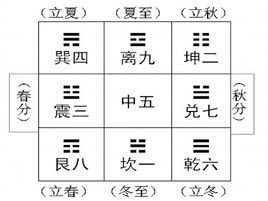
\includegraphics[width=0.3\textwidth]{./figs/chapter3/九宫图}}
\subfigure[河图]{
\label{Fig.sub.2}
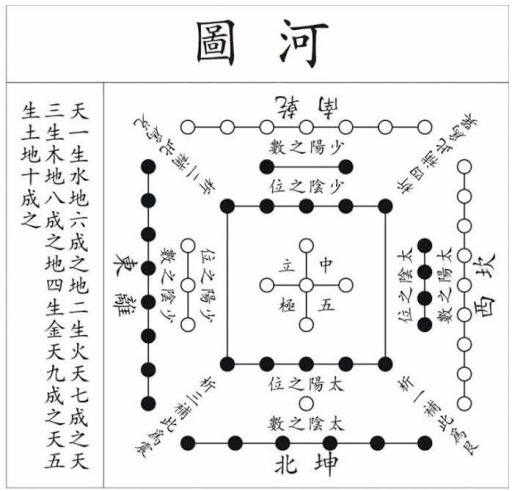
\includegraphics[width=0.3\textwidth]{./figs/chapter3/河图}}
\subfigure[洛书]{
\label{Fig.sub.3}
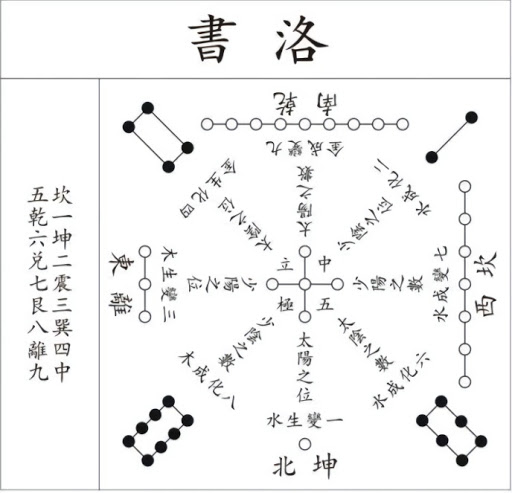
\includegraphics[width=0.3\textwidth]{./figs/chapter3/洛书}}
\caption{九宫图及其起源}
\end{figure}
\indent \textbf{河图}由十种花点组成,分别代表$1-10$这$10$个数,两种花点构成一组,分别布局在东、西、南、北、中五个位置上,每组花点所表示的两个数的差都是$5$。\\
\indent \textbf{洛书}由九种花点组成,分别代表$1-9$这$9$个数,各数的位置排列奇巧,奇偶交替变化,纵横六线及两条对角线上三数之和都为$15$。

\subsection{九宫图问题的求解}
\textbf{口诀一}\\
\indent 九宫者,法以灵龟。二四为肩,六八为足。左三右七,戴九履一,五居中央。\\
\indent \textbf{口诀二}\\
\indent 九子斜列,上下对易,左右相更。四维挺出。
\begin{figure}[H]
\centering
\subfigure[九宫图解一]{
\label{Fig.sub.1}
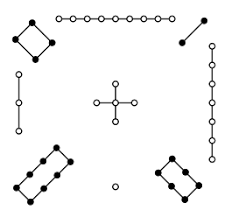
\includegraphics[width=0.2 \textwidth]{./figs/chapter3/九宫图解一}}
\subfigure[九宫图解二]{
\label{Fig.sub.2}
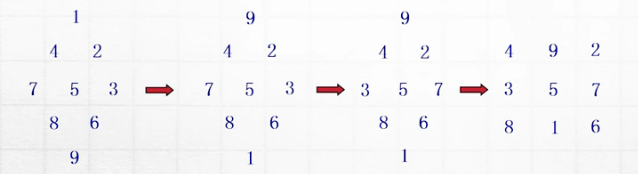
\includegraphics[width=0.6\textwidth]{./figs/chapter3/九宫图解二}}
\caption{九宫图解}
\end{figure}

\section{椅子稳定问题}
\subsection{问题引入与建模准备}
一把四条腿的椅子放在不很平坦的地面上,是否是稳定的?\\
\indent \textbf{不很平坦的定义}:肉眼可见的地面是平坦的\\
\textbf{椅子不稳定的原因}:
\begin{itemize}
\item 椅子的四条腿的长度可能不一样
\item 地面不平坦
\item 椅子的四个底角与地面之间有距离$h,h>0$
\end{itemize}
\indent 三个点确定一个平面,对于相对比较平坦的地面来讲,总可以保证三条腿同时着地,因而只需再使其余的一条腿也能完全着地即可。\\ 
\textbf{量的分析}
\begin{itemize}
\item 椅子的脚和地面的距离作为变量。变量为$0$,意味着椅子的脚与地面没有距离,椅子稳定。
\item 设计旋转角度的连续函数
\end{itemize}

\subsection{模型假设}
\textbf{假设1}:椅子四条腿一样长,椅脚与地面接触处视为一个点,四脚的连线呈正方形$ABCD$,四个椅脚的坐标系中对称;
\begin{figure}[H]
\centering
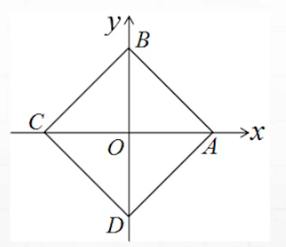
\includegraphics[width=0.3 \textwidth]{figs/chapter3/正方形}
\caption{椅脚坐标系}
\end{figure}

\textbf{假设2}:地面高度使连续变化的,沿任何方向都不会出现间断,如台阶,即地面可视为数学上的连续曲面;\\
\indent \textbf{假设3}:对于椅脚的间距和椅腿长度而言,地面时相对平坦的,使椅子在任何位置至少有三只脚同时着地。


\subsection{模型建立}
\textbf{构造表示距离的函数}:
\begin{itemize}
\item 设$f(\theta)$是$A$、$C$两椅脚与地面的距离之和
\item $g(\theta)$是$B$、$D$两椅脚与地面的距离之和
\item $\theta$是椅子绕中心点$O$旋转角度
\end{itemize}
\begin{figure}[H]
\centering
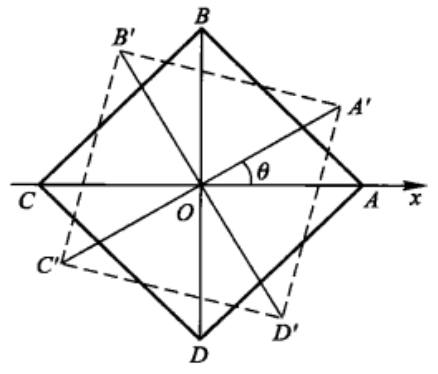
\includegraphics[width=0.3 \textwidth]{figs/chapter3/正方形旋转}
\caption{椅脚坐标系}
\end{figure}
\begin{itemize}
\item 由假设2,$f(\theta)$和$g(\theta)$都是连续函数;
\item 由假设3,椅子在任何位置至少有三只脚同时着地,即对任意的$\theta$,$f(\theta)$和$g(\theta)$中至少有一个为零函数。
\item 在椅子处于初始不稳定的位置时,即$t=0$时,不妨设$g(0)=0,f(0)>0$。
\end{itemize}

\textbf{椅子在不很平坦地面上稳定问题的数学命题}:\\
\indent 已知$f(\theta)$和$g(\theta)$是$t$的连续函数,对任意$\theta$,满足条件$f(\theta) \cdot g(\theta)=0$,且$g(0)=0,f(0)>0$,则至少存在一个$\theta_0$,使$f(\theta_0)=g(\theta_0)=0$,即在旋转椅子的时候,可能在多个位置上都是稳定的。

\subsection{模型求解}
\noindent \textbf{证明}:\\
\indent 将椅子逆时针旋转$\pi\over 2$,则对角线$AC$和$BD$的位置相互交换,且$f(\theta)$和$g(\theta)$是闭区间$[0,{\pi \over 2}]$上的连续函数。\\
\indent 由上面数学命题,一定有下式成立:
\begin{equation}
\begin{cases}
\begin{split}
&g(0)=0,f(0)>0\\
&g({\pi \over 2})>0,f({\pi\over 2})=0
\end{split}
\end{cases}
\end{equation}

\indent 令$h(\theta)=f(\theta)-g(\theta)$,显然$h(\theta)$也是闭区间$[0,{\pi\over 2}]$上的连续函数,\\
\indent 容易检验:$h(\theta)$满足条件$h(0)>0,h({\pi\over 2})<0$。\\
\indent 由闭区间上连续函数的零点存在定理,至少存在$\theta_0$,使得$h(\theta_0)=0$,即$f(\theta_0)=g(\theta_0)$.\\
\indent 再由命题中的条件“对任意$\theta,f(\theta)\cdot g(\theta)=0$”,
得知$f(\theta_0)=g(\theta_0)=0$。

\section{商人过河问题}
\subsection{问题引入}
三个商人各带一名随从渡河,随从们密约:在河的任一岸,一旦随从人数比商人多,就杀人越货。问题:商人该如何设计渡河方案以安全渡河?
\subsection{模型分析}
\noindent \textbf{允许状态集合}\\
\indent $X_k$:第$k$次渡河前此岸的商人数,$X_k,Y_k=0,1,2,3$;\\
\indent $Y_k$:第$k$次渡河前此岸的随从数,$k=1,2,\cdots,n$;\\
\indent 渡河过程的状态:$S_k=(X_k,Y_k)$\\
\indent 允许状态集合:$S=\{(x,y)|x=0,y=0,1,2,3;x=3,y=0,1,2,3;x=y=1,2\}$\\
\textbf{渡河状态集合}\\
\indent $U_k,V_k$:分别任第$k$次渡河船上的商人数与随从数;$(U_k,V_k=0,1,2;k=1,2,\cdots,n)$\\
\indent 决策:$d_k=(U_k,V_k)$\\
\indent 允许决策集合:$D={(u,v)|u+v=1,2}$\\
\textbf {状态转移律}\\
\indent $S_{k+1}=S_k+(-1)^k d_k$
\subsection{模型建立}
制定安全渡河方案归结为如下的多步决策模型:\\
\indent 求$d_k\in D(k=1,2,\cdots,n)$,使$s_k\in S$按状态转移律由$S_1=(3,3)$经有限步$n$到达$S_{n+1}=(0,0)$
\subsection{模型求解}
使用图解法,一共$16$个状态格点,其中允许状态$S$有$10$个点,允许决策$D$表示沿方格移动$1$或$2$格。
\begin{enumerate}[itemindent=2em]
\item [(1).]$k$为奇数,由此岸去彼岸,这时此岸人数减少。移动方向为左/下
\item [(2).]$k$为偶数,由彼岸到此岸,这时此岸人数增多。移动方向为右/上
\item [(3).]$d_k$移动一格表示船上有$1$个人,移动两格表示船上有$2$个人
\item [(4).]用实现表示从此岸去彼岸,虚线表示从彼岸回到此岸
\end{enumerate}
\begin{figure}[H]
\centering
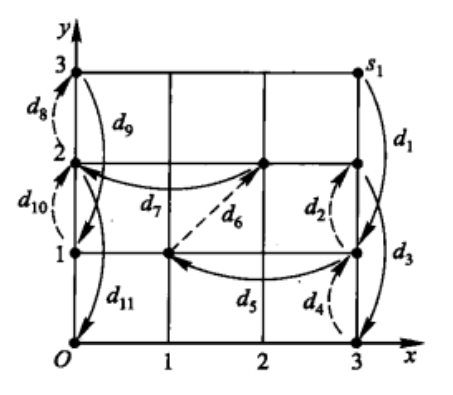
\includegraphics[width=0.45 \textwidth]{figs/chapter3/安全渡河问题图解法}
\caption{安全渡河问题图解法}
\end{figure}


\section{图论方法与网络模型}
\subsection{图论的起源}
图论使组合数学的一个分支,起源于1736年欧拉的第一篇关于图论的论文,这篇论文解决了著名的“哥尼斯堡七桥问题”,从而使欧拉成为图论的创始人。
\subsection{图的概念}
\noindent \textbf{图的定义}\\
\indent 图是一个有序二元组$G={V(G),E(G)}$,其中$V(G)={v_1,v_2,\cdots,v_n}$为顶点集$V(G)$中的元素$v_i$称为顶点,$E(G)={e_1,e_2,\cdots,e_m}$称为边集,$E(G)$中的元素$e_k$叫做边。
\begin{itemize}
\item 顶点总数记位$|V(G)|$,边的总数记位$|E(G)|$
\item 若$|V(G)|=n$,则称$G$为{\bf $n$阶图}
\item 若顶点总数$|V(G)|$与边的总数$|E(G)|$均为有限数,则称$G$为\bf {有限图}
\end{itemize}
\noindent \textbf{有向图的定义}\\
\indent 若顶点集合$V(G)\neq \emptyset$,边集$E(G)\bigcap V(G)=\emptyset$,则称$G=\{V(G),E(G),\emptyset\}$为一个有向图。\\
\noindent \textbf{关联函数}\\
\indent 若$\Phi_G(e)=uv$,$\Phi_G(e)$称为关联函数,表示边$e$与顶点$u$与$v$相关联,又称顶点$u$与$v$相邻,$u$是$e$的尾,$v$是$e$的头,即由$u$指向$v$。\\
\indent 边$e$也成为{\bf 弧},是由两个顶点组成的有序对,通常用尖括号表示。例如:$<v_i,v_j>$,$v_i$称为弧尾,$v_j$称为弧头。$<v_i,v_j>$和$<v_j,v_i>$是两条不同的有向边。\\
\noindent \textbf{无向图的定义}\\
\indent 若$G$的每条边头尾部分,即$\Phi_G(e)=uv=vu$,则称$G$为无向图,无向图中每条边均是顶点的无序对,通常用圆括号表示,例如:$(v_i,v_j)$表示一条无向边,且有$(v_i,v_j)=(v_j,v_i)$。

\subsection{哥尼斯堡七桥问题}
柯尼斯堡七桥问题(Seven Bridges of Königsberg)是图论中的著名问题。这个问题是基于一个现实生活中的事例:当时东普鲁士柯尼斯堡(今日俄罗斯加里宁格勒)市区跨普列戈利亚河两岸,河中心有两个小岛。小岛与河的两岸有七条桥连接。在所有桥都只能走一遍的前提下,如何才能把这个地方所有的桥都走遍?
\begin{figure}[H]
\centering
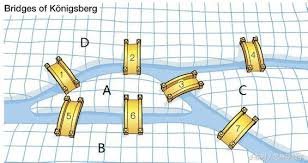
\includegraphics[width=0.6 \textwidth]{figs/chapter3/哥尼斯堡七桥问题}
\caption{哥尼斯堡七桥问题}
\end{figure}
\indent 我们将七桥抽象为无向图中的边,四片陆地抽象为无向图中的点,该无向图可以表示为$G=\{V(G),E(G),\Phi_G\}$,其中$V(G)=\{A,B,C,D\}$,$E(G)=\{a,b,c,d,e,f,g\}$.$\Phi_G(a)=AB$,$\Phi_G(b)=BC$,$\Phi_G(b)=BC$,$\Phi_G(c)=\Phi_G(d)=AC$,$\Phi_G(e)=\Phi_G(f)=AD$,$\Phi_G(g)=BD$。
\begin{figure}[H]
\centering
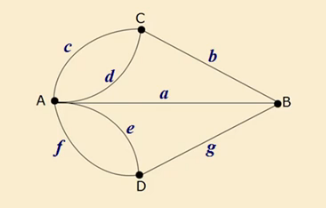
\includegraphics[width=0.6 \textwidth]{figs/chapter3/哥尼斯堡七桥拓扑}
\caption{哥尼斯堡七桥问题图结构}
\end{figure}

\noindent \textbf{七桥问题的图论阐述}\\
\indent 从七桥问题无向图中某个顶点出发,遍历每条边恰好一次,最后能否还回到原来的顶点处(出发点)?


\section{层次分析方法}
\subsection{引子}
\indent 生活中一些问题很难用完全定量的数学模型来解决,对这种复杂决策问题,运用层次分析方法能够找到最佳的解决办法,给出最优的决策。层次分析法(Analytic Hierarchy Process简称AHP)是将与决策有关的元素分解成目标、准则、方案等层次,在此基础上进行定性和定量分析的决策方法。其基本思路与人对一个复杂的决策问题的思维、判断过程大体上是一样的。
\subsection{层次分析法}
\indent 将决策问题按总目标、各层子目标、评价准则直至具体的备选方案的顺序分解为不同的层次结构,然后使用求解判断矩阵特征向量的方法求得每一层次的各元素对上一层次某元素的优先权重,最后再运用加权的方法求出各备选方案对总目标的最终权重向量。其中权重最大者即为最优方案。\\
\indent 层次分析法中每一层的权重设置到最后都会直接或间接影响到结果,而且在每个层次中的每个因素对结果的影响程度都是量化的,非常清晰明确。这种方法擅长于对无结构特性的系统评价以及多目标、多准则、多时期等的系统评价。\\
\indent 层次分析法也具有\textbf{局限性}:
\begin{itemize}
\item 不能为决策提供新方案,层次分析法只能从原有的备选方案中选取最佳方案,因此可能会产生一个由于主观性或者自身创造能力不够而不是最优的方案。
\item 定量数据少,主观因素多,不易令人信服。
\item 指标过多时数据统计量大,且权重难以确定。 当我们希望解决一个具有普适性的问题时,指标的选取数量很可能会随之增加。指标的增加意味着需要构造的层次更深、数量更多、规模更庞大的判断矩阵。
\item 特征值和特征向量的精确求法比较复杂,随着指标的增加,阶数也随之增加,在计算上也变得越来越困难。
\end{itemize}

\subsection{层次分析法的基本步骤}
\noindent 1.{\bf 建立层次结构模型}\\
\indent 在深入分析实际问题的基础上,将有关的各因素按照不同属性自上而下地分解成若干层次,同一层的各个因素因为从属于上一层因素,因此对上层因素会产生较大影响,同时又会支配下一层因素或受到下层因素的影响。\\
\indent 在层次结构模型中,最上层为目标层,通常只有一个因素,最下层通常为方案层,中间可以有一个或几个层次,通常为准则或指标层。当准则过多时(例:$>9$),应进一步分解出子准则层。准则层不宜过少,通常$5-7$个左右。
\begin{figure}[H]
\centering
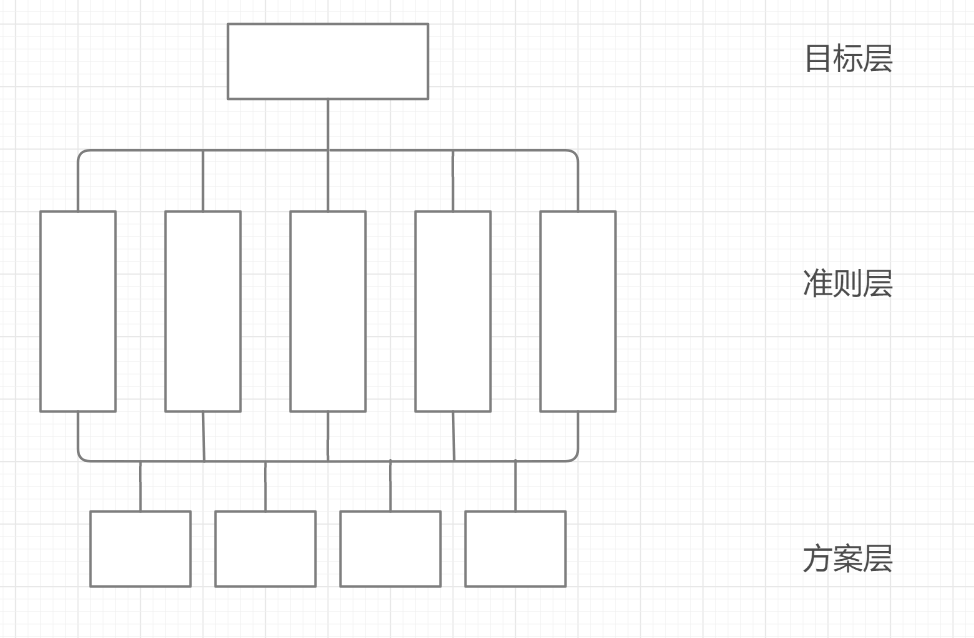
\includegraphics[width=0.6 \textwidth]{figs/chapter3/层次分析结构}
\caption{层次结构模型}
\end{figure}
\noindent 2.{\bf 构造成对比较矩阵}\\
\indent 这一步是要比较层次结构模型的第二层各个因素对上一层因素的影响,从而确定它们对上层因素的影响作用中所占的权重。\\
\indent 设有$n$个因素$x_1,x_2,\cdots,x_n$对上一层目标有影响直接确定它们对目标的影响程度不是很容易,所以每次取两个因素$x_i$与$x_j$比较。用$a_{ij}$表示$x_j$和$x_i$对上层目标的影响比,则$A=(a_{ij})_{m\times n}$称为{\bf 成对比较矩阵},又称为{\bf 正互反矩阵}.
\begin{equation}
A = \left[ {\begin{array}{*{20}{c}}
{\frac{{{x_{\rm{1}}}}}{{{x_1}}}}&{\frac{{{x_1}}}{{{x_2}}}}& \cdots &{\frac{{{x_1}}}{{{x_n}}}}\\
{\frac{{{x_2}}}{{{x_1}}}}&{\frac{{{x_2}}}{{{x_2}}}}& \cdots &{\frac{{{x_2}}}{{{x_n}}}}\\
 \vdots & \vdots & \vdots & \vdots \\
{\frac{{{x_n}}}{{{x_1}}}}&{\frac{{{x_n}}}{{{x_2}}}}& \cdots &{\frac{{{x_n}}}{{{x_n}}}}
\end{array}} \right]_{n\times n},{a_{ij}} > 0,{a_{ii}} = 1,{a_{ij}} = \frac{1}{{{a_{ji}}}}(i = 1,2, \cdots ,n)
\end{equation}
\indent 成对比较矩阵中,每一个$a_{ij}$的取值都是有一定的尺度和规范的,按照Satty的提议,$a_{ij}$在$1-9$及其倒数中间取值。例如:
\begin{itemize}
\item $a_{ij}=1$,元素$i$与元素$j$对上一层次因素的重要性相同
\item $a_{ij}=3$,元素$i$比元素$j$略重要
\item $a_{ij}=5$,元素$i$比元素$j$重要
\item $a_{ij}=7$,元素$i$比元素$j$重要的多
\item $a_{ij}=9$,元素$i$比元素$j$及其重要 
\item $a_{ij}=2,4,6,8$,元素$i$与$j$的重要性介于$1,3,5,7,9$之间
\end{itemize}
\noindent 3.{\bf 计算权向量及一致性检验}\\
\indent 对于每一个成对比较阵计算其最大特征根$\lambda_{max}(A)$及对应特征向量,利用一致性指标、平均随机一致性指标和一致性比率做一致性检验。\\
\indent 若检验通过,那么标准化特征向量即为权向量,若不通过,需要重新构造成对比较阵$A$。\\
\indent 由于成对比较矩阵是我们对复杂事物采取两两比较得到的矩阵,构造过程具有明显的主观性,不可能做到判断具有完全的一致性,难免有误差。所以需要对成对比较矩阵进行一致性检验。\\
\noindent \textbf{定义1}\\
\indent 如果一个正互反矩阵$A$满足$a_{ij}a_{jk}=a_{ik}(i,j,k=1,2,\cdots,n)$则称$A$为一致矩阵,简称一致阵\\
\noindent \textbf{性质1}\\
\indent 如果矩阵$A$是一致阵,那么它的秩为$1$,唯一非零特征根为$n$。\\
\noindent \textbf{性质2}\\
\indent 一致阵的任一列(行)向量都是对应于特征根$n$的特征向量。\\

\noindent \textbf{判别法}\\
\indent 判别一个$n$阶矩阵$A$是否为一致阵,只要计算$A$的最大特征根即可。如果$A$不是一致阵,则可以证明$\lambda_{max}(A)>n$而且$\lambda_{max}(A)>n$越大,说明不一致程度越严重。\\
\noindent \textbf{定义2}\\
\indent 设$\alpha=(\alpha_1,\alpha_2,\cdots,\alpha_n)^T$为正向量,称$\alpha'$为$\alpha$的标准化向量,其中
\begin{equation}
a'=\left( {\frac{{{\alpha_1}}}{{\sum\nolimits_{i = 1}^n {{\alpha_i}} }},\frac{{{\alpha_2}}}{{\sum\nolimits_{i = 1}^n {{\alpha_i}} }}, \cdots ,\frac{{{\alpha_i}}}{{\sum\nolimits_{i = 1}^n {{\alpha_i}} }}} \right)
\end{equation}

\noindent \textbf{一致性检验}\\
设$A$为$n$阶成对比较矩阵
\begin{itemize}
\item {\bf 一致性指标}:$CI={{\lambda-n}\over{n-1}}$来表征一致性程度,当$CI=0$时为一致阵,$CI$越大,$A$的不一致程度越严重。
\item {\bf 平均随机一致性指标}:$RI$来确定$A$的不一致程度的容许范围。对于固定$n$,随机构造成对比较矩阵$A'=(\alpha_{ij}')$其中$a_{ij}'$是从$1,2,\cdots,9$和$1,{1\over 2},\cdots,{1\over 9}$中随机抽取的。这样构造的$A'$是不一致的,它的$CI$相当大。如此构造相当多的$CI$,然后算出这些$A'$的平均值作为平均随机一致性指标的$RI$
\begin{table}[h]
\centering
\caption{随机一致性指标$RI$数值表}
\begin{tabular}{|c|ccccccccccc|}
\hline
{$n$} & $1$ & $2$ & $3$ & $4$ & $5$ & $6$ & $7$ & $8$ & $9$ & $10$ &$11$\\
\hline
{$RI$} & $0$& $0$& $0.58$& $0.90$& $1.12$& $1.24$& $1.32$& $1.41$& $1.45$& $1.49$& $1.51$\\
\hline
\end{tabular}
\end{table}
\item {\bf 一致性比率}:$CR={{CI}\over {RI}}$,当$CR<0.1$时$A$的不一致程度在容许范围内,可用其标准的特征向量$\alpha'$作为权向量,否则需要重新调整判断矩阵$A$
\end{itemize}

\noindent \textbf{权向量的计算方法}
\begin{enumerate}
\item [(1).]如果成对比较矩阵是一致矩阵,则把它的列向量(最大特征根对应的特征向量)标准化得到的向量即为各个因素对上一层目标影响大小的权向量。
\item [(2).]如果成对比较矩阵不是一致矩阵,而它的不一致程度又在容许的范围内,则计算成对比较矩阵的最大特征根及其相对应的特征向量,然后将其标准化,令它作为各个因素对上一层目标影响大小的权向量。
\item [(3).]当成对比较矩阵的不一致程度很严重时,需要重新构造或修正成对比较矩阵。
\end{enumerate}
\noindent \textbf{运用方根法近似计算最大特征值与相应的特征向量}
\begin{enumerate}
\item[(1).] 计算判断矩阵每一行元素的乘积 ${W_i} = \prod\limits_{j = 1}^n {{a_{ij}}(i,j = 1,2, \cdots ,n)}$
\item[(2).]计算$W_i$的$n$次方根${\bar W_i} = \sqrt[n]{{{W_i}}}$
\item[(3).] 对向量${\bar W_i} = ({\bar W_1},{\bar W_2}, \cdots {\bar W_n})$做标准化处理${a_i} = {\bar W_i} \div \sum\limits_{j = 1}^n {{{\bar W}_j}(i = 1,2, \cdots ,n)}$,得到${B=(a_1,a_2,\cdots,a_n)^T}$即为所求的特征向量
\item[(4).] 计算最大特征值${\lambda _{\max }}(A) = \frac{1}{n}\sum\limits_{i = 1}^n {\frac{{{{(AB)}_i}}}{{{a_i}}}}$,其中
\begin{equation}\nonumber
AB{\rm{ = }}\left[ {\begin{array}{*{20}{c}}
{{{(AB)}_1}}\\
{{{(AB)}_2}}\\
 \vdots \\
{{{(AB)}_N}}
\end{array}} \right] = \left[ {\begin{array}{*{20}{c}}
{{a_{{\rm{11}}}}}&{{a_{12}}}& \cdots &{{a_{1n}}}\\
{{a_{21}}}&{{a_{22}}}& \cdots &{{a_{2n}}}\\
 \vdots & \vdots & \vdots & \vdots \\
{{a_{n1}}}&{{a_{n2}}}& \cdots &{{a_{nn}}}
\end{array}} \right] \cdot \left[ {\begin{array}{*{20}{c}}
{{a_1}}\\
{{a_2}}\\
 \vdots \\
{{a_n}}
\end{array}} \right]
\end{equation}
上式中,$(AB)_i$表示向量$AB$的第$i$个元素
\end{enumerate}

\noindent4.{\bf 计算组合权向量并做组合一致性检验}\\
\indent 这是层次分析法的最后一个步骤,需要计算最下层对最上层目标的组合权向量,并做组合一致性检验。若检验通过,则可按照组合权向量表示的结果进行决策,否则需要重新考虑模型或重新构造那些一致性比率较大的成对比较矩阵。
\subsection{假期旅游案例}
\noindent \textbf{问题描述}\\
\indent 假如你在准备一趟假期旅游,有三个景点A、B、C供你选择,你将根据景点费用、居住条件、饮食和旅途等准则比较这三个候选景点,并最终决策选择其中一个景点。\\
\noindent \textbf{层次结构模型}
\begin{figure}[H]
\centering
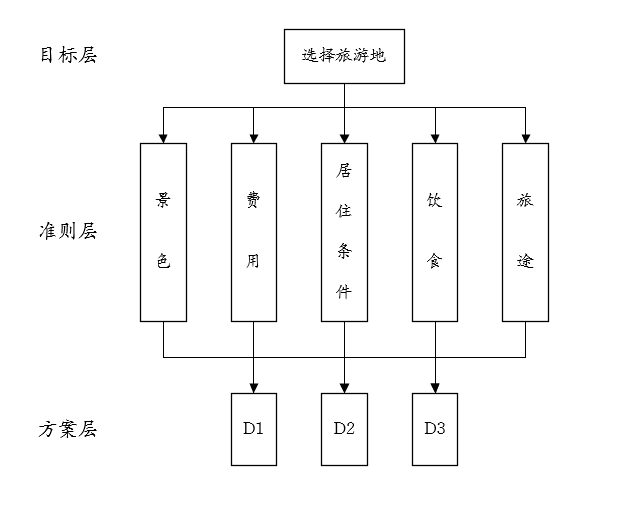
\includegraphics[width=0.6 \textwidth]{figs/chapter3/旅游地选择层次分析模型}
\caption{旅游地选择层次分析模型}
\end{figure}
\noindent \textbf{构造成对比较矩阵}\\
\indent 设景色、费用、居住条件、饮食和交通便利五个因素分别为$X_1$,$X_2$,$X_3$,$X_4$,$X_5$,假设成对比较矩阵如下:
\begin{equation}\nonumber
A = \left[ {\begin{array}{*{20}{c}}
1&{\frac{1}{2}}&4&3&3\\
2&1&7&5&5\\
{\frac{1}{4}}&{\frac{1}{7}}&1&{\frac{1}{2}}&{\frac{1}{3}}\\
{\frac{1}{3}}&{\frac{1}{5}}&2&1&1\\
{\frac{1}{3}}&{\frac{1}{5}}&3&1&1
\end{array}} \right]
\end{equation}
\indent 其中$a_{21}=2$表示费用$X_2$与景色$X_1$对选择旅游地这个目标的比是$2:1$,说明对费用看的更重要一些,其他同理。\\
\noindent \textbf{计算权向量与一致性检验}\\
\indent 运用上一节的方法计算可得最大特征值$\lambda_{max}=5.073$,一致性指标$CI={{\lambda_{max}-n}\over{n-1}}={{5.073-5}\over{5-1}}=0.018$,查表得$RI=1.12$,最终可得一致性比率$CR={{CI}\over{RI}}={0.018\over 1.12}=0.016<0.1$,因此通过了一致性检验。\\
\indent 计算特征根$\lambda_{max}=5.073$对应的特征向量并对其标准化,得$\alpha=\alpha^{(2)}=(0.263,0.475,0.055,0.099,0.110)^T$,为了跟后面得步骤进行区分,这里记位$\alpha^{(2)}$。\\
\indent 从向量中可以看出费用最为重要,其次是景色和旅途,再次是饮食和居住条件。

\noindent \textbf{计算组合权向量并做一致性检验}\\
\indent 三个方案分别针对五个准则构造成对比较矩阵,如下:
\begin{equation}\nonumber
{B_1} = \left[ {\begin{array}{*{20}{c}}
1&2&5\\
{\frac{1}{2}}&1&2\\
{\frac{1}{5}}&{\frac{1}{2}}&1
\end{array}} \right] \quad
{B_2} = \left[ {\begin{array}{*{20}{c}}
1&{\frac{1}{3}}&{\frac{1}{8}}\\
3&1&{\frac{1}{3}}\\
8&3&1
\end{array}} \right] \quad
{B_3} = \left[ {\begin{array}{*{20}{c}}
1&1&3\\
1&1&3\\
{\frac{1}{3}}&{\frac{1}{3}}&1
\end{array}} \right] \quad
{B_4} = \left[ {\begin{array}{*{20}{c}}
1&1&4\\
{\frac{1}{3}}&1&1\\
{\frac{1}{4}}&1&1
\end{array}} \right] \quad
{B_5} = \left[ {\begin{array}{*{20}{c}}
1&1&{\frac{1}{4}}\\
1&1&{\frac{1}{4}}\\
4&4&1
\end{array}} \right]
\end{equation}
\indent $B_1,B_2,B_3,B_4,B5$表示三种旅游方案$D_1,D_2,D_3$分别对准则层中的五个因素(景色、费用、居住条件、饮食和旅途)的影响程度的比较矩阵。例如$B_3$中的$b_{23}=3$表示方案$D_2$与$D_3$相比居住条件好坏的程度之比。\\
\indent 接着分别计算各矩阵的最大特征根以及相应的权向量,再经过标准化得到标准化向量,然后我们还需要对他们分别进行一致性检验,结果如下表:
\begin{table}[h]
\centering
\caption{数值表}
\begin{tabular}{|c|c|c|c|c|c|}
\hline
{$k$} & $1$ & $2$ & $3$ & $4$ & $5$ \\
\hline
{$\alpha_k^{(3)}$}& {$\begin{array}{*{20}{c}}0.595\\ 0.277\\ 0.129\end{array}$} & {$\begin{array}{*{20}{c}}0.082\\0.236\\0.682\end{array}$} & 
{$\begin{array}{*{20}{c}}0.429\\ 0.429\\ 0.142\end{array}$} & {$\begin{array}{*{20}{c}}0.633\\ 0.193\\ 0.175\end{array}$} & {$\begin{array}{*{20}{c}}0.166\\0.166\\0.668\end{array}$}  \\
\hline
{$\lambda_k$}&3.005 &3.002 & 3 & 3.009 & 3\\
\hline
{${CI}_{k}$}&0.003 &0.001 & 0 &0.005 & 0\\
\hline 
{${CR}_k$}&0.052 &0.002 &0 &0.009 & 0 \\
\hline
\end{tabular}
\end{table}
\\
\indent 显然,这5个矩阵都通过了一致性检验,其中$\alpha_k^{(3)}$即为组合权向量,表示第二层对第一层以及第三层对第二层各个因素的综合影响。\\
\indent 最终我们需要的组合权向量$\alpha^{(3)}=\alpha_k^{(3)}\times \alpha^{(2)})=(0.300,0.246,0.456)^T$,即表示三个景点$D_1,D_2,D_3$中分别占的比重,所以可知方案$D_3$占有更高的比重,因此应该选择方案$D_3$。
\section{双层玻璃问题}
\subsection{问题的提出}
\indent 来自北方的同学可能会知道,身边很多的玻璃窗都是双层的,两层玻璃之间是真空的空隙。那么这样的工艺有什么好处呢?它可以有效的阻止室内温度想室外的扩散。那么当建筑物室内外的热传递过程处于热力学平衡状态时,这种构造形式的双层玻璃窗究竟能比单层玻璃窗阻止多少热量损失?两层玻璃窗之间的距离控制在多少为好?
\subsection{量的分析}
\noindent\textbf{符号说明}
\begin{table}[htbp]
\centering
\caption{符号表}
\begin{tabular}{|c|l|}
\hline
符号 & 说明 \\
\hline
{$T_1$} & 室内温度\\
{$T_2$} & 室外温度\\
{$d$} & 单层玻璃温度\\
{$l$} & 两层玻璃之间的空气温度\\
{$T_a$} & 内层玻璃的外侧温度\\
{$T_b$} & 外层玻璃的内测温度\\
{$k$} & 热传导系数\\
{$Q$} &热量损失\\
\hline 
\end{tabular}
\end{table}
\subsection{模型假设}
\begin{enumerate}
\item 热量的传播过程只有传导没有对流,即窗户的密封性能良好,两层玻璃之间的空气是不流动的
\item 室内温度和室外温度保持不变,热传导过程已处于稳定状态即沿热传导方向,单位时间内通过单位面积的热量是常熟
\item 玻璃材料均匀,热传导系数是常数
\begin{figure}[H]
\centering
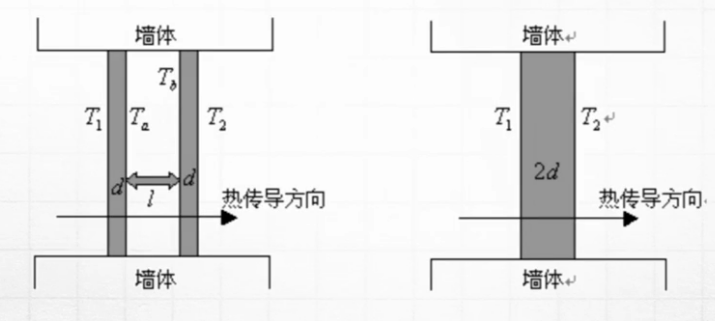
\includegraphics[width=0.6 \textwidth]{figs/chapter3/玻璃热传导示意图}
\caption{玻璃热传导示意图}
\end{figure}
\end{enumerate}
\subsection{模型建立}
\noindent \textbf{热力学传导定律}\\
\indent 厚度为$d$的均匀介质,两侧温度差为$\Delta T$,则单位时间由温度高的一侧向温度低的一侧通过单位面积的热量$Q$与温度差$\Delta T$成正比,与介质的厚度$d$成反比,即
\begin{equation}
Q=k{{\Delta T}\over d}
\end{equation}
\indent 其中,$k$为热传导系数。\\
\noindent \textbf{双层玻璃的热量流失}\\
\indent 由热传导方程遵从的物理定律得知
\begin{equation}
Q=k_1{{T_1-T_a}\over d}=k_2{{T_a-T_b}\over l}=k_1{{T_b-T_2}\over d}
\end{equation}
\indent 由(3.7)式,可知
\begin{equation}
T_1-T_a=T_b-T_2={{dQ}\over k_1},T_a-T_b={{lQ}\over k_2}
\end{equation}
\indent 从而得到
\begin{equation}
T_1-T_2=(T_1-T_a)+(T_a+T_b)+(T_b-T_2)=({{{2d}\over k_1}+{l\over{k_2}}})Q
\end{equation}
\indent 由此可知
\begin{equation}
Q={{k_1(T_1-T_2)}\over{d(s+2)}},s=h{k_1\over k_2},h={l\over d}
\end{equation}

\noindent \textbf{单层玻璃的热量流失}\\
\indent 对于厚度为$2d$的单层玻璃窗户,其热量流失为
\begin{equation}
Q'=k_1{{T_1-T_2}\over{2d}}
\end{equation}
\noindent \textbf{单层玻璃窗和双层玻璃窗热量流失比较}\\
\indent 由$(3.7)$式和$(3.11)$式,可知:
\begin{equation}
{Q\over Q'}={2\over{s+2}}<1
\end{equation}
\indent 因此可见,双层玻璃窗热量流失一定是小于单层玻璃窗的。\\
\indent 已知不流通、干燥空气的热传导系数是$k_2=2.5\times 10^{-4}(J/cm\cdot s\cdot\mbox{度} )$,常用玻璃的热传导系数是$k_1=4\times 10^{-3}-8\times 10^{-3}(J/cm\cdot s\cdot \mbox{度})$,于是${k_1\over k_2}\in[16,32]$。\\
\indent 在分析双层玻璃窗比单层玻璃窗可减少多少热量损失时,我们做最保守的估计,即取$k_1\over k_2$的最小值16,由$(3.7)$式和$(3.11)$式可得:
\begin{equation}
{Q\over Q'}={1\over{8h+1}},h={l\over d}
\end{equation}
\subsection{模型分析与求解}
\indent 比值${Q\over Q'}=(8h+1)^{-1}$反映了双层玻璃窗在减少热量损失的功效,它只与$h={l\over d}$有关。
\begin{figure}[H]
\centering
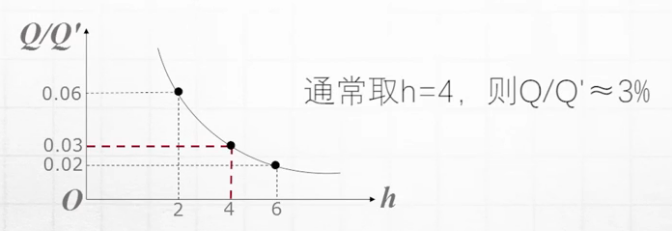
\includegraphics[width=0.6 \textwidth]{figs/chapter3/热量损失比重}
\caption{热量损失比重示意图}
\end{figure}
\indent 通过描述曲线,我们可以观察到$h=4$时,${Q\over Q'}\approx 3\%$,即$Q\approx 3\% Q'$,也就是说双层玻璃窗热量损耗是单层玻璃窗的$3\%$,换句话说双层玻璃窗能够阻止$97\%$的热量,要比单层玻璃窗的功效更好。从图中可以看到,从$h=4$往后,曲线的走势趋于平缓,减少热量损失的功效不明显,因此实际操作时可以建议操作者,双层玻璃窗之间的厚度和玻璃之间的比值控制在$4$倍即可。

\chapter{微积分与微分方程方法建模}
\section{Malthus人口模型}
\subsection{Malthus人口论}
\noindent \textbf{Malthus指数增长模型}\\
\indent 反映人口增加与食物增加速度之间的关系,是刻画单种群模型的典型代表,被世界公认为“马尔萨斯人口论”\\
\noindent \textbf{马尔萨斯人口理论主要论点}\\
\indent 生活资料按$1、2、3、4、5\cdots$的算术级数增加,而人口是按$1、2、4、8、16\cdots$几何级数增长,因此生活资料的增加赶不上人口的增长,这是自然的永恒的规律。\\
\noindent \textbf{重要假设}\\
\indent 大规模种群的个体数量是时间的连续可微函数。\\
\indent 设$x(t)$是$t$时刻的人口总数量,种群个体总数的变化主要受出生、死亡、迁入和迁出等因素的影响。假设种群是孤立的,即不考虑迁入迁出因素,那么种群的繁衍发展就不受其他生物种群的影响。

\subsection{基本概念}
\noindent \textbf{人口自然增长率}\\
\indent 一定时期内人口自然增加数与同一时期平均人口之比,即:
\begin{equation}
\mbox{人口自然增长率}={{\mbox{一年内人口自然增长率}}\over {\mbox{年平均人口数}}}
\end{equation}
\noindent \textbf{人口平均增长率}\\
\indent 一定时期内人口增加量与期初数和所用时间乘积之比,即:
\begin{equation}
\mbox{人口平均增长率}={{\mbox{期末人口总数}-\mbox{期初人口总数}}\over{\mbox{期初人口数}\times\mbox{所用时间}}}
\end{equation}
\noindent \textbf{人口增长率}\\
\indent 人口平均增长率在所用时间趋于零时的极限,即:
\begin{equation}
r(t) = \mathop {\lim }\limits_{\Delta t \to 0} \frac{{x(t + \Delta t) - x(t)}}{{\Delta t \times x(t)}}
\end{equation}
\indent 其中$x(t)$为$t$时刻的人口总数量。
\subsection{模型假设}
\begin{itemize}[itemindent=2em]
\item 假设1:人口发展过程比较平稳(这是建模工作的基本要求);
\item 假设2:人口数量为时间的连续可微函数,即人口的取值在整数集合上的离散变量,不是连续的量。但是由于通常人口数量很庞大,为了运用微积分工具,将离散问题做连续化处理;
\item 假设3:人口增长率是与时间$t$无关的常数$r$,该假设是对欧洲百余年人口数据做统计研究作出的,是一种近似。
\end{itemize}
\subsection{模型建立与求解}
\indent 根据假设$(3)$,人口增长率$r$为与时间无关的常数,即任意时刻$t$,均有:
\begin{equation}
\mathop {\lim }\limits_{\Delta t \to 0} \frac{{x(t + \Delta t) - x(t)}}{{\Delta t \times x(t)}}=r(r\mbox{为常数})
\end{equation}
\indent 再根据假设$(2)$,$x(t)$为时间的连续可微函数,可得$x(t)$满足以下微分方程:
\begin{equation}
\begin{cases}
{{dx}\over{dt}}=rx\\
x(0)=x_0
\end{cases}
\end{equation}
\indent 运用分离变量法,容易求得上述常微分方程的解为
\begin{equation}
x(t)={x_0}e^{rt}
\end{equation}
\indent 容易看出,当$t\to\infty $时,人口总数将趋于无穷大,即
\begin{equation}
\mathop {\lim}\limits_{t\to\infty}x(t)=\mathop {\lim}\limits_{t\to \infty} {x_0}e^{rt}=\infty
\end{equation}
\subsection{应用案例}
\indent 以美国$1790-1930$年的人口统计资料为数据依据:
\begin{figure}[H]
\centering
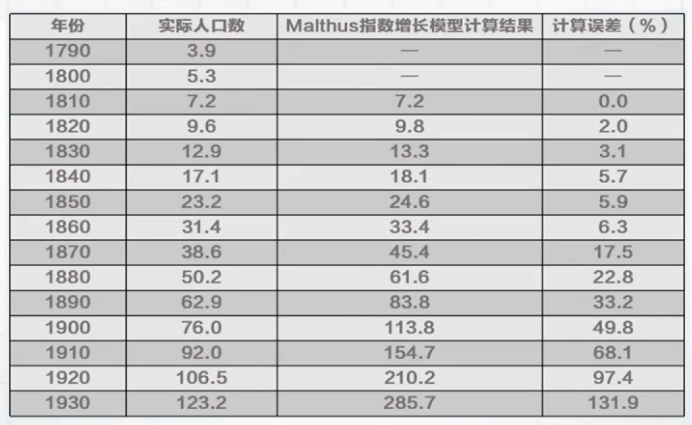
\includegraphics[width=0.6 \textwidth]{figs/chapter4/美国人口统计数据}
\caption{美国1790-1930年人口统计数据\quad 单位:百万}
\end{figure}
\indent 通过这张表,我们可以看出,在短期内的表现Malthus人口模型的拟合还是比较吻合的,但是随着时间的推移,长期来看,误差越来越大。为什么会出现这样的误差呢?我们慢慢来分析。\\
\indent 要想构造Malthus人口模型,我们首先就要通过给出的资料来计算人口增长5率。假设增长率$r$是常数,我们将$x(0)=3.9,x(1)=5.3$,代入人口指数增长模型中,计算人口增长率$r$:
\begin{equation}
r={{lnx(1)-lnx(0)}\over{t}}={{ln5.3-ln3.9}\over{10}}={{1.66771-1.36098}\over{10}}\approx 0.03067
\end{equation}
\noindent \textbf{结果分析}:\\
\indent 种群规模和时间跨度小,符合实际;种群规模和时间跨度大,误差较大。若$r>0$,当$t\to +\infty$时,有$x(t)\to +\infty$,因此,该模型不能用于对人口的长期预测。\\
\indent 原因就出在{\bf 假设$3$},$r$是常数没有考虑有限的资源对种群的增长会产生阻滞作用。因此如果要更好的预测长期的种群增长情况,我们一定要考虑地球有限的资源会给种群增长带来什么样的影响。因此我们需要对Malthus人口模型进行修正。\\
\indent 人口的增加必定会消耗有限的资源,因此有限的资源必定会限制人口的增长,这种现象必将促使人口增长率的下降,也就是说,{\bf 人口增长率是人口数量的递减函数}。我们将据此对Malthus模型进行修正,这种修正的结果是我们将得到一个另外的反映人口变动的模型,叫做Logistic模型。
\subsection{Logistic阻滞增长模型}
\indent P.F.Verhulst引入环境的最大容量常数$Xmax$,简记为$Xm$,表示自然资源和环境条件下所能容许的最大人口数量,而且为了进一步的考虑资源环境对种群的规模增长所产生的这种阻滞的影响作用,Verhulst又增加了以下几条假设:
\begin{itemize}
\item{假设4}:确定的环境内的资源供给为常数,且对每个个体的分配是均等的,即表明当种群规模(密度)增大时,每个个体食物的平均分配量必然减少,从而导致种群增长率降低。
\item{假设5}:种群个体的增长率是$x(t)$的线性减函数,即为:
\begin{equation}
r-r{{x(t)}\over{x_m}}=r{1-{x(t)\over{x_m}}}(x_m>x(t)>0)
\end{equation}
\end{itemize}
\indent 当$x(t)=X_m$时,种群规模不再增大,$X_m$代表环境所能容许的种群最大数量,得到种群增长的 Verhulst阻滞增长模型:
\begin{equation}
\begin{cases}
\frac{{dx}}{{dt}} = r\left[ {1 - \frac{{x(t)}}{{{x_m}}}} \right]x(t)\\
x(0)=x_0
\end{cases}
\end{equation}
\indent 其中$1-{{x(t)}\over {x_m}}$叫做$Verhulst$因子,$-{r\over{x_m}}x^2{(t)}$反映种群密度对种群规模增长的抑制作用,称为密度制约。不考虑密度制约时就是原来的Malthus模型\\
\noindent\textbf{Logistic模型的解}\\
\indent 模型(4.10)即为Logistic模型,其解为:
\begin{equation}
x(t)={{x_m}\over{1+({{x_m}\over{x_0}}-1)e^{-rt}}}
\end{equation}
\begin{figure}[H]
\centering
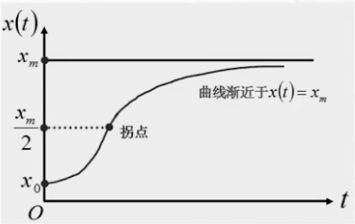
\includegraphics[width=0.45 \textwidth]{figs/chapter4/Verhulst人口模型}
\caption{Verhulst人口模型}
\end{figure}
\noindent\textbf{人口总量与人口对时间变化率的关系}:
\begin{figure}[H]
\centering
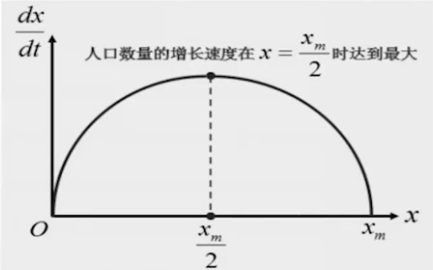
\includegraphics[width=0.45 \textwidth]{figs/chapter4/人口总量与人口对时间变化率的关系}
\caption{人口总量与人口对时间变化率的关系}
\end{figure}
\indent 由图可知,$0-{{X_m}\over 2}$时,增长率是单调递增的,当$x={{X_m}\over 2}$时,增长率达到最大,当$x=X_m$时,增长率为$0$。
\section{细菌的繁殖数学模型}
\subsection{问题的提出}
\indent 已知某时刻某种细菌的数量,预测在任意时刻$t$这种细菌的数量变化趋势,建立细菌繁殖的数学模型。
\subsection{模型假设}
\indent 由实验可知,细菌繁殖的速度应该和培养基是否充足。当培养基充足时,细菌繁殖的速度$V$与当时已有的数量$A_0$成正比,即$y=kA_0(k>0\mbox{为比例常数})$
\begin{itemize}
\item 假设某种细菌的个数按照指数方式增长,给出如下表:
\begin{table}[htbp]
\centering
\caption{细菌繁殖数据表}
\begin{tabular}{|c|c|}
\hline
天数 & 细菌个数 \\
\hline
{$5$} & $936$\\
\hline
{$10$} & $2190$\\
\hline 
\end{tabular}
\end{table}
\item 假设在每一个小时间段$[{{(i-1)}\over n}t,{i\over n}t](i=1,2,\cdots,n)$内细菌的繁殖速度不变,且在各小段时间内只繁殖一次。
\end{itemize}
\indent 按照假设,我们要求的是:
\begin{enumerate}[itemindent=2em]
\item [(1).]开始时细菌的个数可能是多少?
\item [(2).]若继续以现在速度增长下去,假定细菌无死亡,那么60天后细菌的个数应该是多少?
\end{enumerate}

\subsection{模型建立}
\indent 首先我们要量化这个数学模型,设细菌总数为$y$,为了计算出$t$时刻细菌的个数,我们需要将时间间隔$[0,t]$分成$N$等分,通过对细菌数量的变化来着手研究细菌的繁衍速度问题。\\
\indent 细菌的繁殖过程可视为连续变化的,在很短的一段时间内数量的变化很小,繁殖的速度可以近似地看作不变。由假设$(2)$在第一段时间$[0,{t\over n}]$内,细菌繁殖的数量为${kA_0t}\over n$\\
\indent 第一段时间末细菌的数量为$A_0(1+{{kt}\over n})$;\\
\indent 第二段时间末细菌的数量为$A_0(1+{{kt}\over n})^2$;\\
\indent 依此类推,到最后一段时间末细菌的数量为
\begin{equation}
y=A_0(1+k{t\over n})^n
\end{equation}
\noindent\textbf{结论}
\indent 时间间隔无限细分(即$n\to\infty$)时,可求得精确值,经过时间t后细菌的总数是:
\begin{equation}
\begin{split}
A_0\mathop {\lim }\limits_{n \to \infty } {\left( {1 +{k \cdot {t\over {n}}}} \right)^n}&= A_0 \mathop {\lim }\limits_{n \to \infty } {\left( {1 + {{kt}\over n}} \right)^n}\\
&= A_0\mathop {\lim }\limits_{n \to \infty } {\left[ {{{\left( {1 + \frac{1}{x}} \right)}^x}} \right]^{kt}}\\
&={A_0}{\left[ {\mathop {\lim }\limits_{x \to \infty } {{\left( {1 + \frac{1}{x}} \right)}^x}} \right]^{kt}}\\
&={A_0}{e^{kt}}
\end{split}
\end{equation}
\indent 至此我们得到细菌繁殖服从生长函数模型:
\begin{equation}
y=A_0e^{kt}
\end{equation}
\indent 其中,$k$为繁衍比例系数,$t$为时间,$A_0$为细菌初始数量。
\subsection{模型求解}
\indent 由公式$(4.14)$及题目所给数据表$4.1$得:
\begin{equation}
\begin{cases}
936=A_0e^{5k}\\
2190=A_0e{10k}
\end{cases}
\end{equation}

\indent 解此方程组,得$A_0=400,k=0.17$.即开始时细菌个数为$400$个
\indent 按此速度增长下去,则60天后细菌个数为:
\begin{equation}\nonumber
y(60)=400e^{60\times 0.17}\approx 10761200(\mbox{个})
\end{equation}


\section{传染病流行的控制模型}
\indent 通常某种传染病的大面积流行,例如伤风、流感等,最常见的传播方式是带菌患者通过空气、食物和饮食等渠道,把病菌传播给健康人,形成传播锁链。
\subsection{传统的传染病流行控制模型}
\indent 假设$t$时刻的病人数目$x(t)$是时间$t$的连续可微函数,每天每个病人有效接触(足以使被接触者致病)的人数为常数$k$,考察$t$到$t+\Delta t$发病人数的增加,再假设$t=t_0$时有$x_0$个病人,即得微分方程
\begin{equation}
x(t+\Delta{t)}-x(t)=k\cdot x(t)\cdot\Delta{t})
\end{equation}
\begin{equation}
{{dx}\over{dt}}=kx(t),x(t_0)=x_0
\end{equation}
\indent 将这个模型对比前面学习过得Malthus指数增长模型,可以看出二者非常相似,这个模型得解与Malthus指数增长模型的解是完全一样的\\
\noindent\textbf{模型的结果分析}\\
\indent 随着时间$t$的增加,患病人数$x(t)$将无限增加,不符合实际,模型建立失败\\
\noindent\textbf{原因分析}\\
\indent 病人有效接触的人群中既有健康人也有已经发病的人,只有健康人才可以被传染而成为患病的人,建模需要区分人群。
\subsection{改进的传染病流行控制模型(SI模型)}
\subsubsection{模型假设}
\begin{itemize}
\item 在疾病传播期内,所考察地区的总人数$N$不变,既不考虑生死,也不考虑迁移。
\item 把人群$N$分为易感染者和已感染者两类,简称健康者和病人。在$t$时刻这两类人在总人数中所占的比例分别记作$x(t)$和$y(t)$。
\item 每个病人每天有效接触的平均人数是常数$k$,$k$称为日接触率。假设当病人与健康者进行有效接触时,可使健康者受到感染成为病人。
\end{itemize}
\subsubsection{模型建立}
\indent 每个病人每天可使$kx(t)$人感染成为病人,病人数为$N\cdot y(t)$,每天有$kx(t)Ny(t)$个健康者被感染。
\begin{itemize}
\item 病人数$N\cdot y(t)$对时间的增长率为
\begin{equation}
{{d(Ny)}\over{dt}}=k\cdot x(t)\cdot N\cdot y(t)
\end{equation}
\item 初始时刻$t=0$,病人的比例记位$y(0)=y_0$
\end{itemize}
\indent 得到改进的$SI$模型:
\begin{equation}
\begin{cases}
{{dy}\over{dt}}=k\cdot y(t)\cdot{[N-y(t)]}\\
y(0)=y_0\\
N=x(t)+y(t)=1
\end{cases}
\end{equation}
\indent 这依然是一个微分方程的初值问题,其实它就是本章第一节所讲的改进的Logistic模型,即{\bf 阻滞增长模型}
\subsubsection{模型求解}
\begin{equation}
y(t)={{N}\over{1+{\left({N\over y_0}-1\right)\cdot e^{-kt}}}}
\end{equation}
\subsubsection{结果分析}
\indent 负指数函数$e^{-kt}(k>0)$起到了衰减作用,因此$t$越来越大(发病持续的时间逐渐增加)时,$e^{-kt}$将越来越小,因此$1+{\left({N\over y_0}-1\right)}\cdot e^{-kt}$也将越来越小,从而$y(t)$随$t$的增大单调增加。因此当$t\to\infty$时,$\mathop{\lim}\limits_{t\to\infty}{y(t)}=N$。
\begin{itemize}[itemindent=2em]
\item 当已感染者达到总人数的一半,即$y=0.5$时,${dy}\over{dt}$达到最大值,很容易求出这个时刻为$t_m=k^{-1}ln\left( {1\over{y_0}-1}\right)$,表明此时刻病人增加的速度最快。可以认为这是医院门诊量最大的时刻,预示着传染病爆发高潮的到来,需要医疗卫生部门高度关注。
\item 由$t_m=k^{-1}ln\left( {1\over{y_0}-1}\right)$得知,$t_m$与$k$成反比例关系,原因是模型中的日接触率表示该地区的医疗卫生水平的高低,$k$越小,表明卫生水平越高。因此,改善保健设施,提高卫生与防御水平可以推迟传染病爆发高潮的到来时间。
\item 由SI模型解的表达式(4.20)可以看出,$y(t)$随$t$单调增加,$t\to\infty$时有$\mathop{\lim}\limits_{t\to\infty}y(t)=N$,这说明所有的人最终都将被传染,全部成为病人,不符合实际情况。
\end{itemize}
\subsection{病人得到治愈的SIS模型}
在上一节的结果分析指出,SI模型解的表达式不符合实际情况。为什么这么说呢?因为SI模型没有考虑到病人还可以被治愈成为健康者,存在思考上的缺陷。
\indent 有些传染病被治愈后会使患者的免疫力非常低,因此可以假设没有免疫性,于是病人被治愈后成为健康者,但是健康者还有可能再次被感染,再次成为病人。这个模型称为SIS模型。
\subsubsection{模型假设}
\begin{itemize}
\item 在疾病传播期内,所考察地区的总人数$N$不变,既不考虑生死,也不考虑迁移。
\item 把人群$N$分为易感染者和已感染者两类,简称健康者和病人。在$t$时刻这两类人在总人数种所占的比例分别记作$x(t)$和$y(t)$。
\item 每天被治愈的病人数占病人总数的比例为常数$\lambda$,称为日治愈率。病人治愈后成为仍可被感染的健康者。$1\over\lambda$是这种传染病的平均传染期。
\end{itemize}
\subsubsection{模型建立}
\begin{equation}
\begin{cases}
N{{dy}\over{dt}}=k\cdot N\cdot x(t)\cdot y(t)-\lambda\cdot N\cdot y(t)\\
x(t)+y(t)=1
\end{cases}
\end{equation}
\indent 经过整理,得到:
\begin{equation}
\begin{cases}
{{dy}\over{dt}}=k\cdot y(t)\cdot [N-y(t)]\\
y(0)=y_0
\end{cases}
\end{equation}
\noindent \textbf{定义} $\sigma={k\over\lambda}$,其中$k$是每个病人有效接触(足以使被接触者致病)的人数,$1\over\lambda$是这种传染病的平均传染期。$\sigma$的含义是整个传染期内的每个病人有效接触的平均人数,简称接触数。
\subsubsection{模型求解分析}
\indent 利用定义$\sigma=k\over \lambda$,SIS模型可以改写成:
\begin{equation}
{{dy}\over{dt}}=-ky(t)\left[y(t)-\left(1-{1\over\sigma} \right) \right]
\end{equation}
\subsubsection{SIS模型的结论}
\indent 接触数$\sigma=1$是一个阈值(临界值),讨论如下:
\begin{itemize}[itemindent=2em]
\item $\sigma$>1时,$y(t)$的增减性取决于$y_0$的大小,其极限值$\mathop{\lim}\limits_{t\to\infty}y(t)=1-{1\over\sigma}$随$\sigma$的增加而增加。
\item 当$\sigma\le 1$时,病人比例$y(t)$越来越小,最终趋于零。这是由于传染期内经有效接触从而使健康者变为病人数不超过原来病人数的缘故。
\end{itemize}

\section{价格数学模型}
\subsection{价格数学模型的定义}
价格数学模型是运用数学的方法对价格形成和价格变动规律所作的描述。最常见的是投入-产出价格数学模型
\subsection{价格数学模型的分类}
\begin{itemize}
\item 从价格形成的内在机制上来描述经济变量种的数量关系
\item 从经济事物表面现象上探索经济变量间的内在联系
\item 组合模型
\end{itemize}
\subsection{价格数学模型的分析}
\subsubsection{一些概念}
\begin{itemize}
\item 均衡价格是指商品的供给与需求相等时的市场价格
\item 实际的市场价格通常不会等于均衡价格,并且随时间不断变化
\end{itemize}
\indent 假设在某一时刻$t$,某商品的价格与该商品的均衡价格有差别,此时会存在供需差,供需差必将促使价格变动
\subsection{价格数学模型的建立}
\indent 设某商品在时刻$t$的销售价格为$p(t)$,市场对该商品的需求量和它对市场的供给量分别为$D(p)$、$S(p)$,它们均为价格$p$的函数。\\
\indent 在$t$时刻价格$p(t)$对时间$t$的变化率${dp}\over{dt}$与该商品在同一时刻市场超额需求量$D(p)-S(p)$成正比,即
\begin{equation}
{{dp}\over{dt}}=k\left[ D(p)-S(p)\right](k>0,\mbox{为比例系数})
\end{equation}
\indent 由经济学原理可知,商品供给量$S(p)$是价格$p$的单调递增函数,而市场需求量$D(p)$是价格$p$的单调递减函数。假设
\begin{equation}
S(p)=a+bp,D(p)=c-dp
\end{equation}
\indent 其中$a$、$b$、$c$、$d$均为正的常数。当供给量$S(p)$与需求量$D(p)$相等时,对应的价格便是均衡价格$p^*$。\\
\indent 那么当供给量与需求量相等时
\begin{equation}\nonumber
a+bp=c-dp
\end{equation}
\indent 这表示两条曲线$S(p)=a+bp$与$D(p)=c-dp$的交点恰好为供求平衡时的均衡价格$p^*$,即
\begin{equation}
p^*=(c-a)\div(d+b)
\end{equation}
\indent 当商品供不应求时,即$S(p)<D(p)$,商品价格要上涨\\
\indent 当商品供过于求时,即$S(p)>D(p)$,商品价格要下降\\
\indent 将(4.25)式代入(4.24)式中,得
\begin{equation}
{{dp}\over{dt}}=\alpha(p^*-p)
\end{equation}
\indent 其中,$\alpha=k(b+d)>0$,另方程(4.27)得通解是:
\begin{equation}
p(t)=p^*+Ce^{-\alpha t}
\end{equation}
\indent 假设初始价格为$p(0)=p_0$,代入上式,得$C=p_0-p^*$,从而得到价格表达式
\begin{equation}
p(t)=p^*+(p_0-p^*)e^{-\alpha t}
\end{equation}
\indent 由$\alpha >0$时,当$t\to\infty$时,$e^{-\alpha t}\to\infty$,因而价格将趋近于均衡价格,即$p(t)\to{p^*}$
\subsection{结论}
\indent 随着时间不断延续,市场价格将逐渐趋近于均衡价格$p^*$
\section{湖泊污染减退模型}
\subsection{模型的背景介绍}
\indent 随着世界经济的迅猛发展,水污染问题日益加剧,水体的污染最突出的问题就是富营养化。根据联合国环境规划署(UNEP)的一项调查表明全球范围内的湖泊和水库30\%-40\%都有不同程度的富营养化现象。
\subsubsection{湖泊富营养化的特点}
\begin{itemize}
\item 发展速度快
\item 危害程度大
\item 治理过程难
\item 修复历时长
\end{itemize}
\indent\indent 数学模型可以综合反映系统特征,因此建立该问题的数学模型是针对湖泊污染管理工作种特别有用的手段。
\subsubsection{湖泊富营养化研究模型的种类}
\begin{enumerate}
\item {\bf 经验回归模型}:经验回归模型是在多年实测水质浓度资料及相关环境资料,如生物数据的基础上,进行多元回归分析建立起的经验模型。大多用来描述叶绿素和磷与透明度之间的关系。也可用来预测浮游植物生物量,藻类平均与最大生物量之间的关系。由于自身的缺点,通常只在数据不太理想或建立复杂模型前用作初步的半定量估计。
\item {\bf 营养盐模型}:主要用来研究引起富营养化的营养物质,主要是碳、氮、磷,一般淡水环境中三者的比率为$106:16:1$
\item {\bf 浮游植物动力学模型}:浮游藻类的生长是富营养化的关键过程,研究氮、磷负荷与浮游藻类生产力的相互作用和关系是揭示湖泊富营养化形成机理的主要途径
\item {\bf 生态系统动力学模型}:研究湖泊的生态结构、功能、时空演变规律及其物理、化学、生物过程对水生生态系统的影响及其反馈机制
\end{enumerate}
\subsection{问题的提出}
\indent 如果在某个时刻污染物质停止进入湖里,那么需要多长时间,能使湖水的污染浓度下降到污染刚刚停止时污染浓度的5\%?
\subsection{模型假设}
\begin{enumerate}
\item 把湖泊视为一个单一的流入、流出系统。
\item 湖水中的污染物质均匀分布在水域里,不存在局部湖水中污染物浓度高于其他区域的现象。
\item 湖水体积视为一个常数。
\item 模型中各个变量是连续变化并且充分光滑的。
\item 不考虑生物学自身反应或变化导致的污染物在水域中的自行消亡现象,即污染物质除了流出湖水外,不会因自身发生某些生物化学反应、沉积、死亡或其他各种方式而自尽自灭。
\end{enumerate}
\subsection{模型的建立与求解}
\indent 假设某湖水的体积$V$不变,记$x(t)$为任一时刻$t$每立方米湖水所含污染物质的数量(即污染程度的度量),$r$为每天流出湖里的水量(立方米),则由假设3(湖水的体积是常数)得知$r$也是每天流入湖里的水量
\subsubsection{解决该问题的方法依赖以下事实}
污染物质对时间的变化率=单位时间内流入湖中的污染物质-单位时间内流出湖中的污染物质,即
\begin{equation}
{{d}\over{dt}}[x(t)\cdot V]=0-r\cdot x(t)\quad (r,V\mbox{为常数})
\end{equation}
\indent 得到污染减退的数学模型,如下
\begin{equation}
V{{dx}\over{dt}}=-rx \quad \mbox{或}\quad {1\over x}\cdot{{dx}\over{dt}}={-{r\over V}}
\end{equation}
\indent 利用分离变量法,再积分,求得该问题的解为
\begin{equation}
x(t)=x(0)e^{-{r\over V}t}
\end{equation}
\indent 当$x(t)=5\%x(0)$时,有$5\%x(0)=x(0)e^{-{r\over V}t}$,两边取对数,整理得$t_{0.05}\approx{{3V}\over r}$
\subsection{结论}
\indent 本模型的建立是在非常简单的假设条件下的一个很粗糙的模型。事实上江河湖海的污染问题是各种各样、复杂多变的。污染物质的减退不仅仅靠湖水多年来自然流动,蒸发和渗漏也是不可忽视的因素,另外不同的污染物质对湖水污染的影响大小也是存在差异的。

\chapter{线性规划模型}
\section{线性规划模型实例}
\section{线性规划问题}
\section{求解线性规划问题的基本思想}
\section{线性规划问题的几何解释和图解法}
\section{整数线性规划问题}
\section{线性规划的对偶理论}
\section{非对称形式的对偶线性规划问题}
\section{两铁路平板车的装货问题}

\chapter{对策模型}
\section{对策模型的引入}
\section{对策模型的基本理论}
\section{矩阵对策模型}
\section{矩阵对策模型实例分析}
\section{鞍点存在定理}
\section{混合对策模型}

\chapter{决策模型}
\section{决策模型的概念及分类}
\section{风险型决策}
\section{不确定型决策}
\bookmarksetup{startatroot}
\part{数学建模思想}
\chapter{预测与预报}
\section{灰色预测模型}
$P1\_20min$
\section{微分方程预测}
\section{回归分析预测}
\section{马尔科夫预测}
\section{时间序列预测}
\section{小波分析预测}
\section{神经网络预测}
\section{混沌序列预测}
\chapter{评价与决策}
\section{模糊综合评价}
\section{主成分分析}
\section{层次分析法(AHP)}
\section{因子分析}
\section{数据包络(DEA)分析法}
\section{秩和比综合评价法}
\section{优劣解距离法(TOPSIS)}
\section{投影寻踪综合评价法}
\section{方差分析与协方差分析}
\chapter{聚类和判别}
\section{距离聚类(常用)}
\section{关联性聚类(常用)}
\section{层次聚类}
\section{密度聚类}
\section{其他聚类}
\section{贝叶斯判别(统计判别方法)}
\section{费舍尔判别(训练样本较多)}
\section{模糊识别(分好类的数据点较少)}
\chapter{关联与因果}
\section{灰色关联分析方法}
\section{Sperman或kendall等级相关分析}
\section{Person相关}
\section{Copula相关}
\section{典型相关分析}
\section{标准化回归分析}
\section{生存分析(事件史分析)}
\section{格兰杰因果检验}
\chapter{优化与控制}
\section{线性规划、整数规划、0-1规划}
有约束,确定的目标
\section{非线性规划与智能优化算法}
\section{多目标规划}
柔性约束,目标含糊
\section{动态规划}

\section{网络优化}
多因素交错复杂
\section{排队论与计算机仿真}
\section{模糊规划}
范围约束
\section{灰色规划}
\part{数学建模算法}
\chapter{蒙特卡洛算法}
\chapter{数据处理算法}
\chapter{规划类算法}
\chapter{图论算法}
\chapter{计算机算法}
\chapter{智能优化算法}
\chapter{网格算法与穷举算法}
\chapter{一些离散化算法}
\chapter{数值分析算法}
\chapter{图像处理算法}


\part{数据预处理}
\part{数据可视化}
\chapter{可视化基础}
\section{绪论}
\section{字体}
\section{颜色}
\chapter{统计图表}
\section{线型图}
\subsection{简单的线型图}
\lstinputlisting[
    style       =   Python,
    caption     =   {\bf SimpleLine.py},
    label       =   {SimpleLine.py}
]{code/lines/SimpleLine.py}
\begin{figure}[H]
\centering
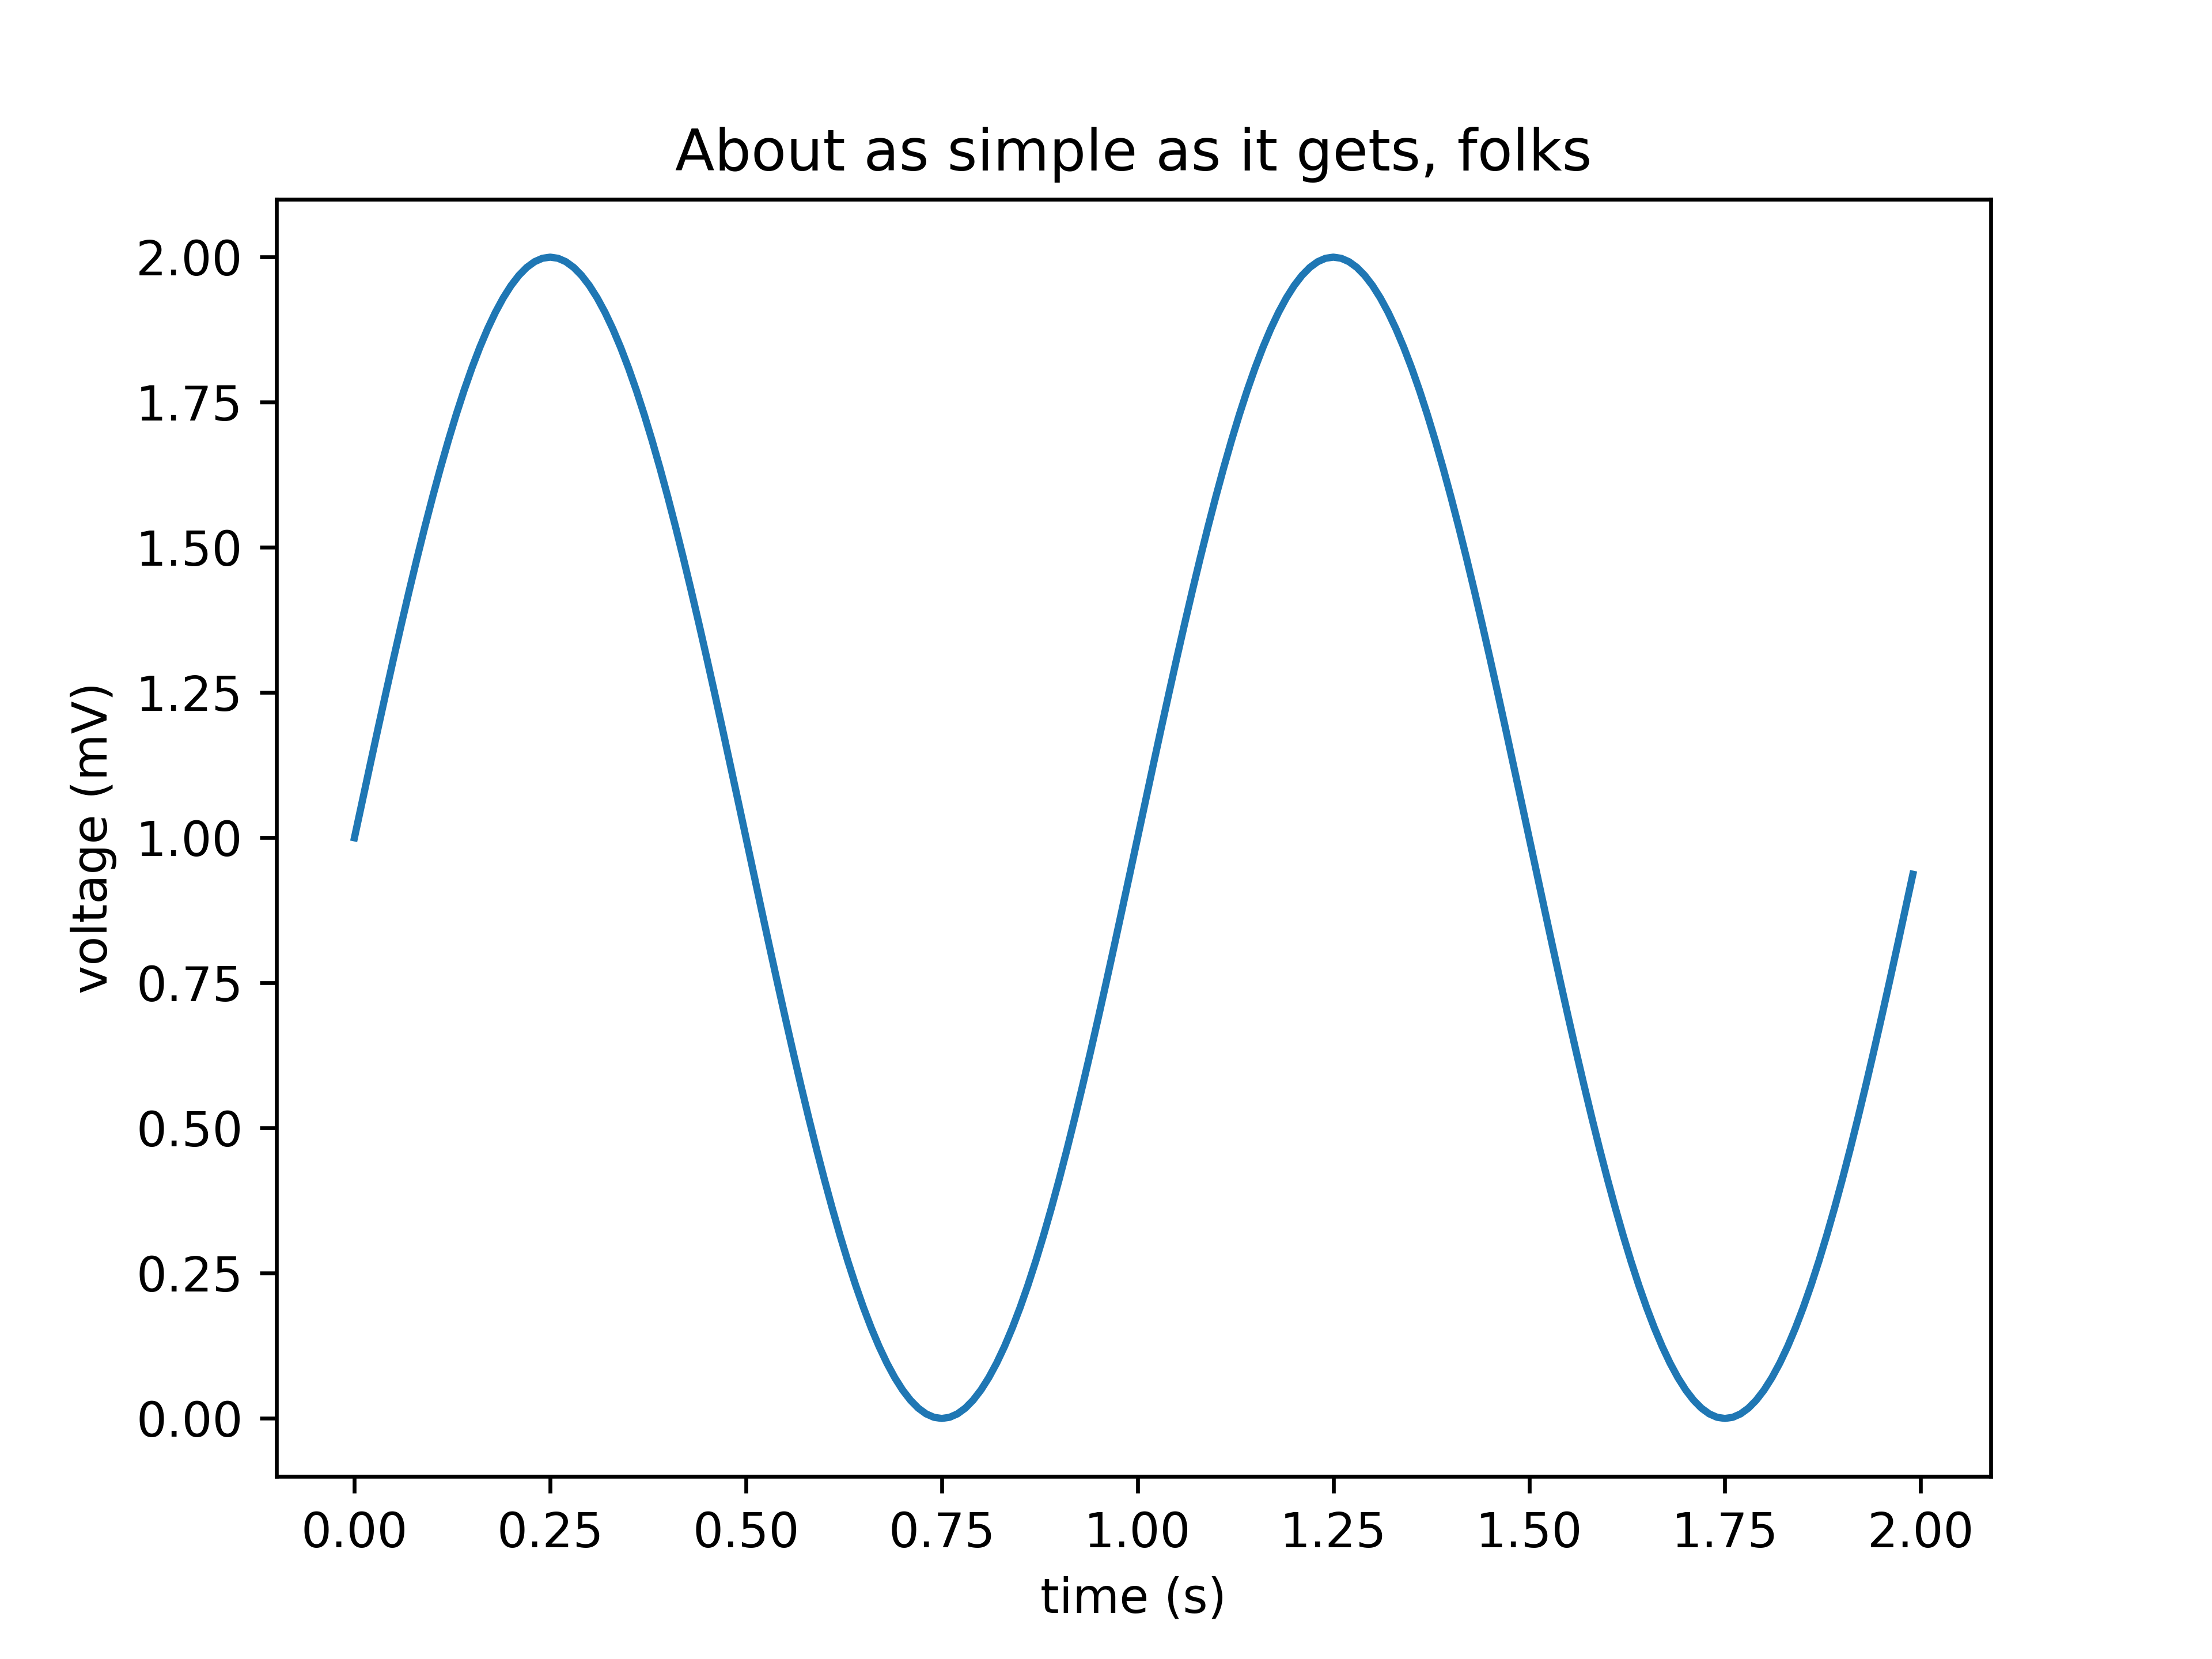
\includegraphics[width=0.6 \textwidth]{figs/chapter9/lines/SimpleLine}
\caption{简单的线型图}
\end{figure}

\subsection{自定义虚线样式}
\lstinputlisting[
    style       =   Python,
    caption     =   {\bf CustomizeLineStyle.py},
    label       =   {CustomizeLineStyle.py}
]{code/lines/CustomizeLineStyle.py}
\begin{figure}[H]
\centering
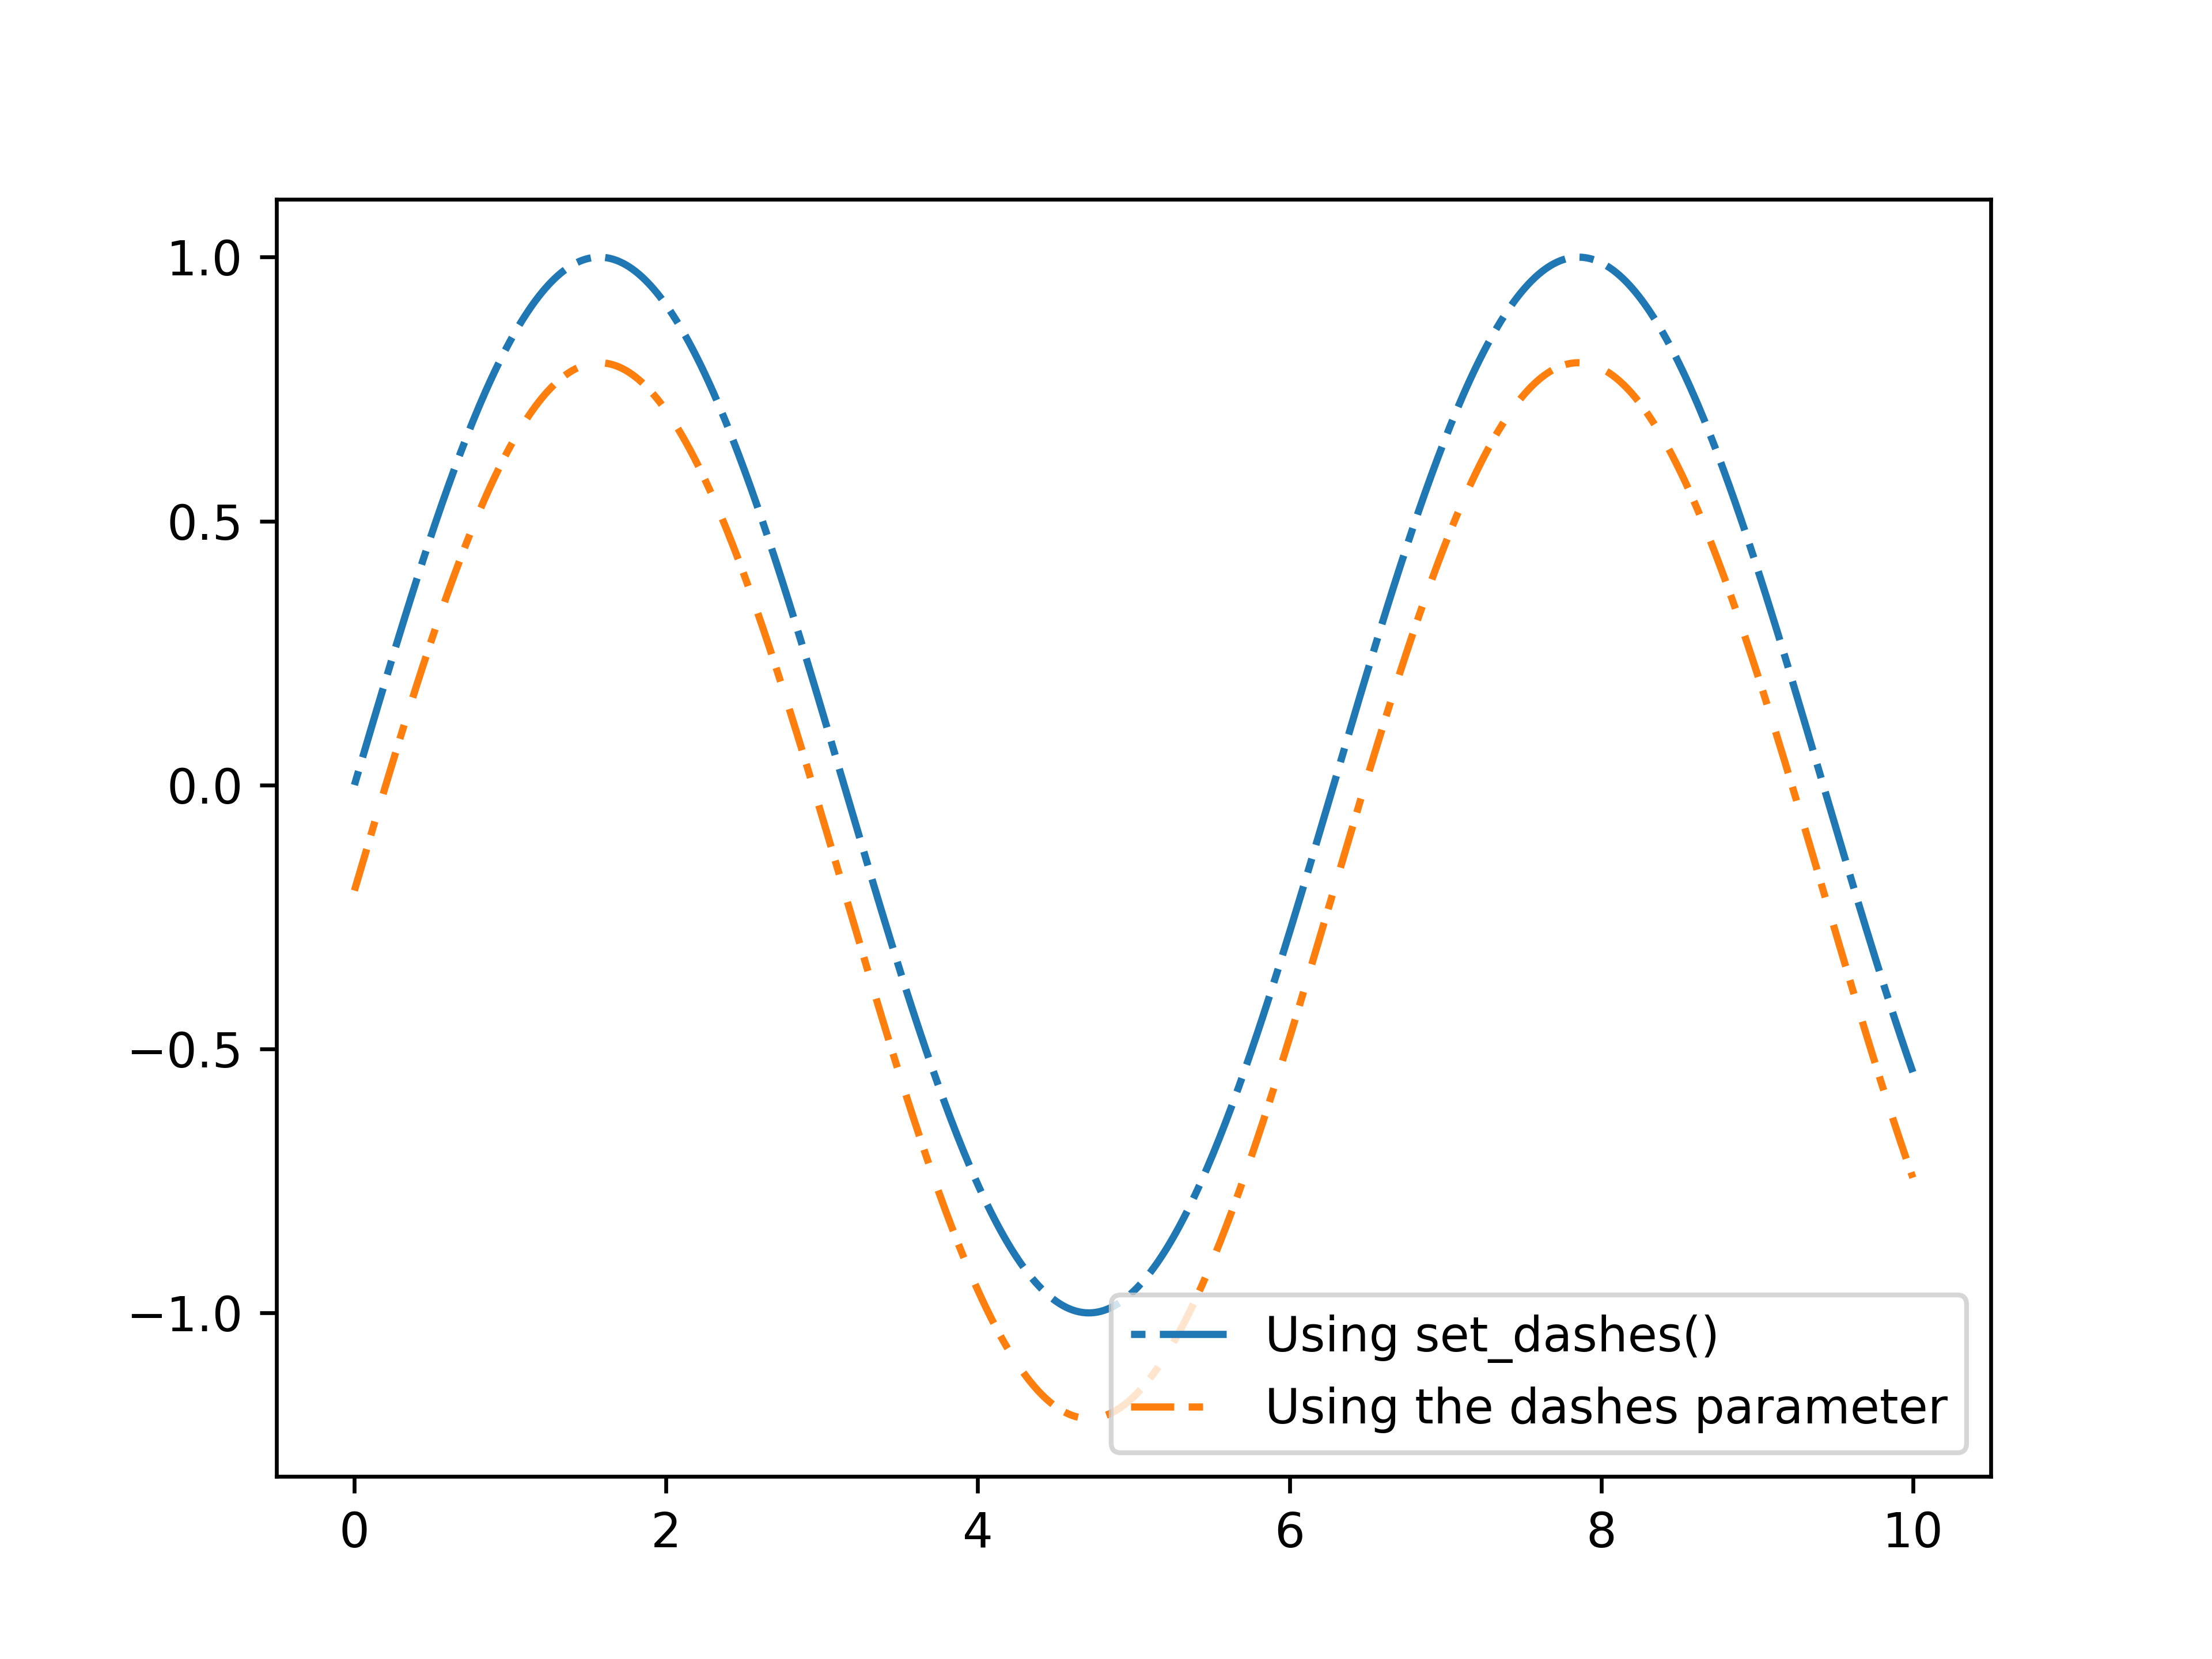
\includegraphics[width=0.6 \textwidth]{figs/chapter9/lines/CustomizeLineStyle}
\caption{自定义虚线样式}
\end{figure}
\subsection{误差限制选择线}
\lstinputlisting[
    style       =   Python,
    caption     =   {\bf UpLowErrorBar.py},
    label       =   {UpLowErrorBar.py}
]{code/lines/UpLowErrorBar.py}
\begin{figure}[H]
\centering
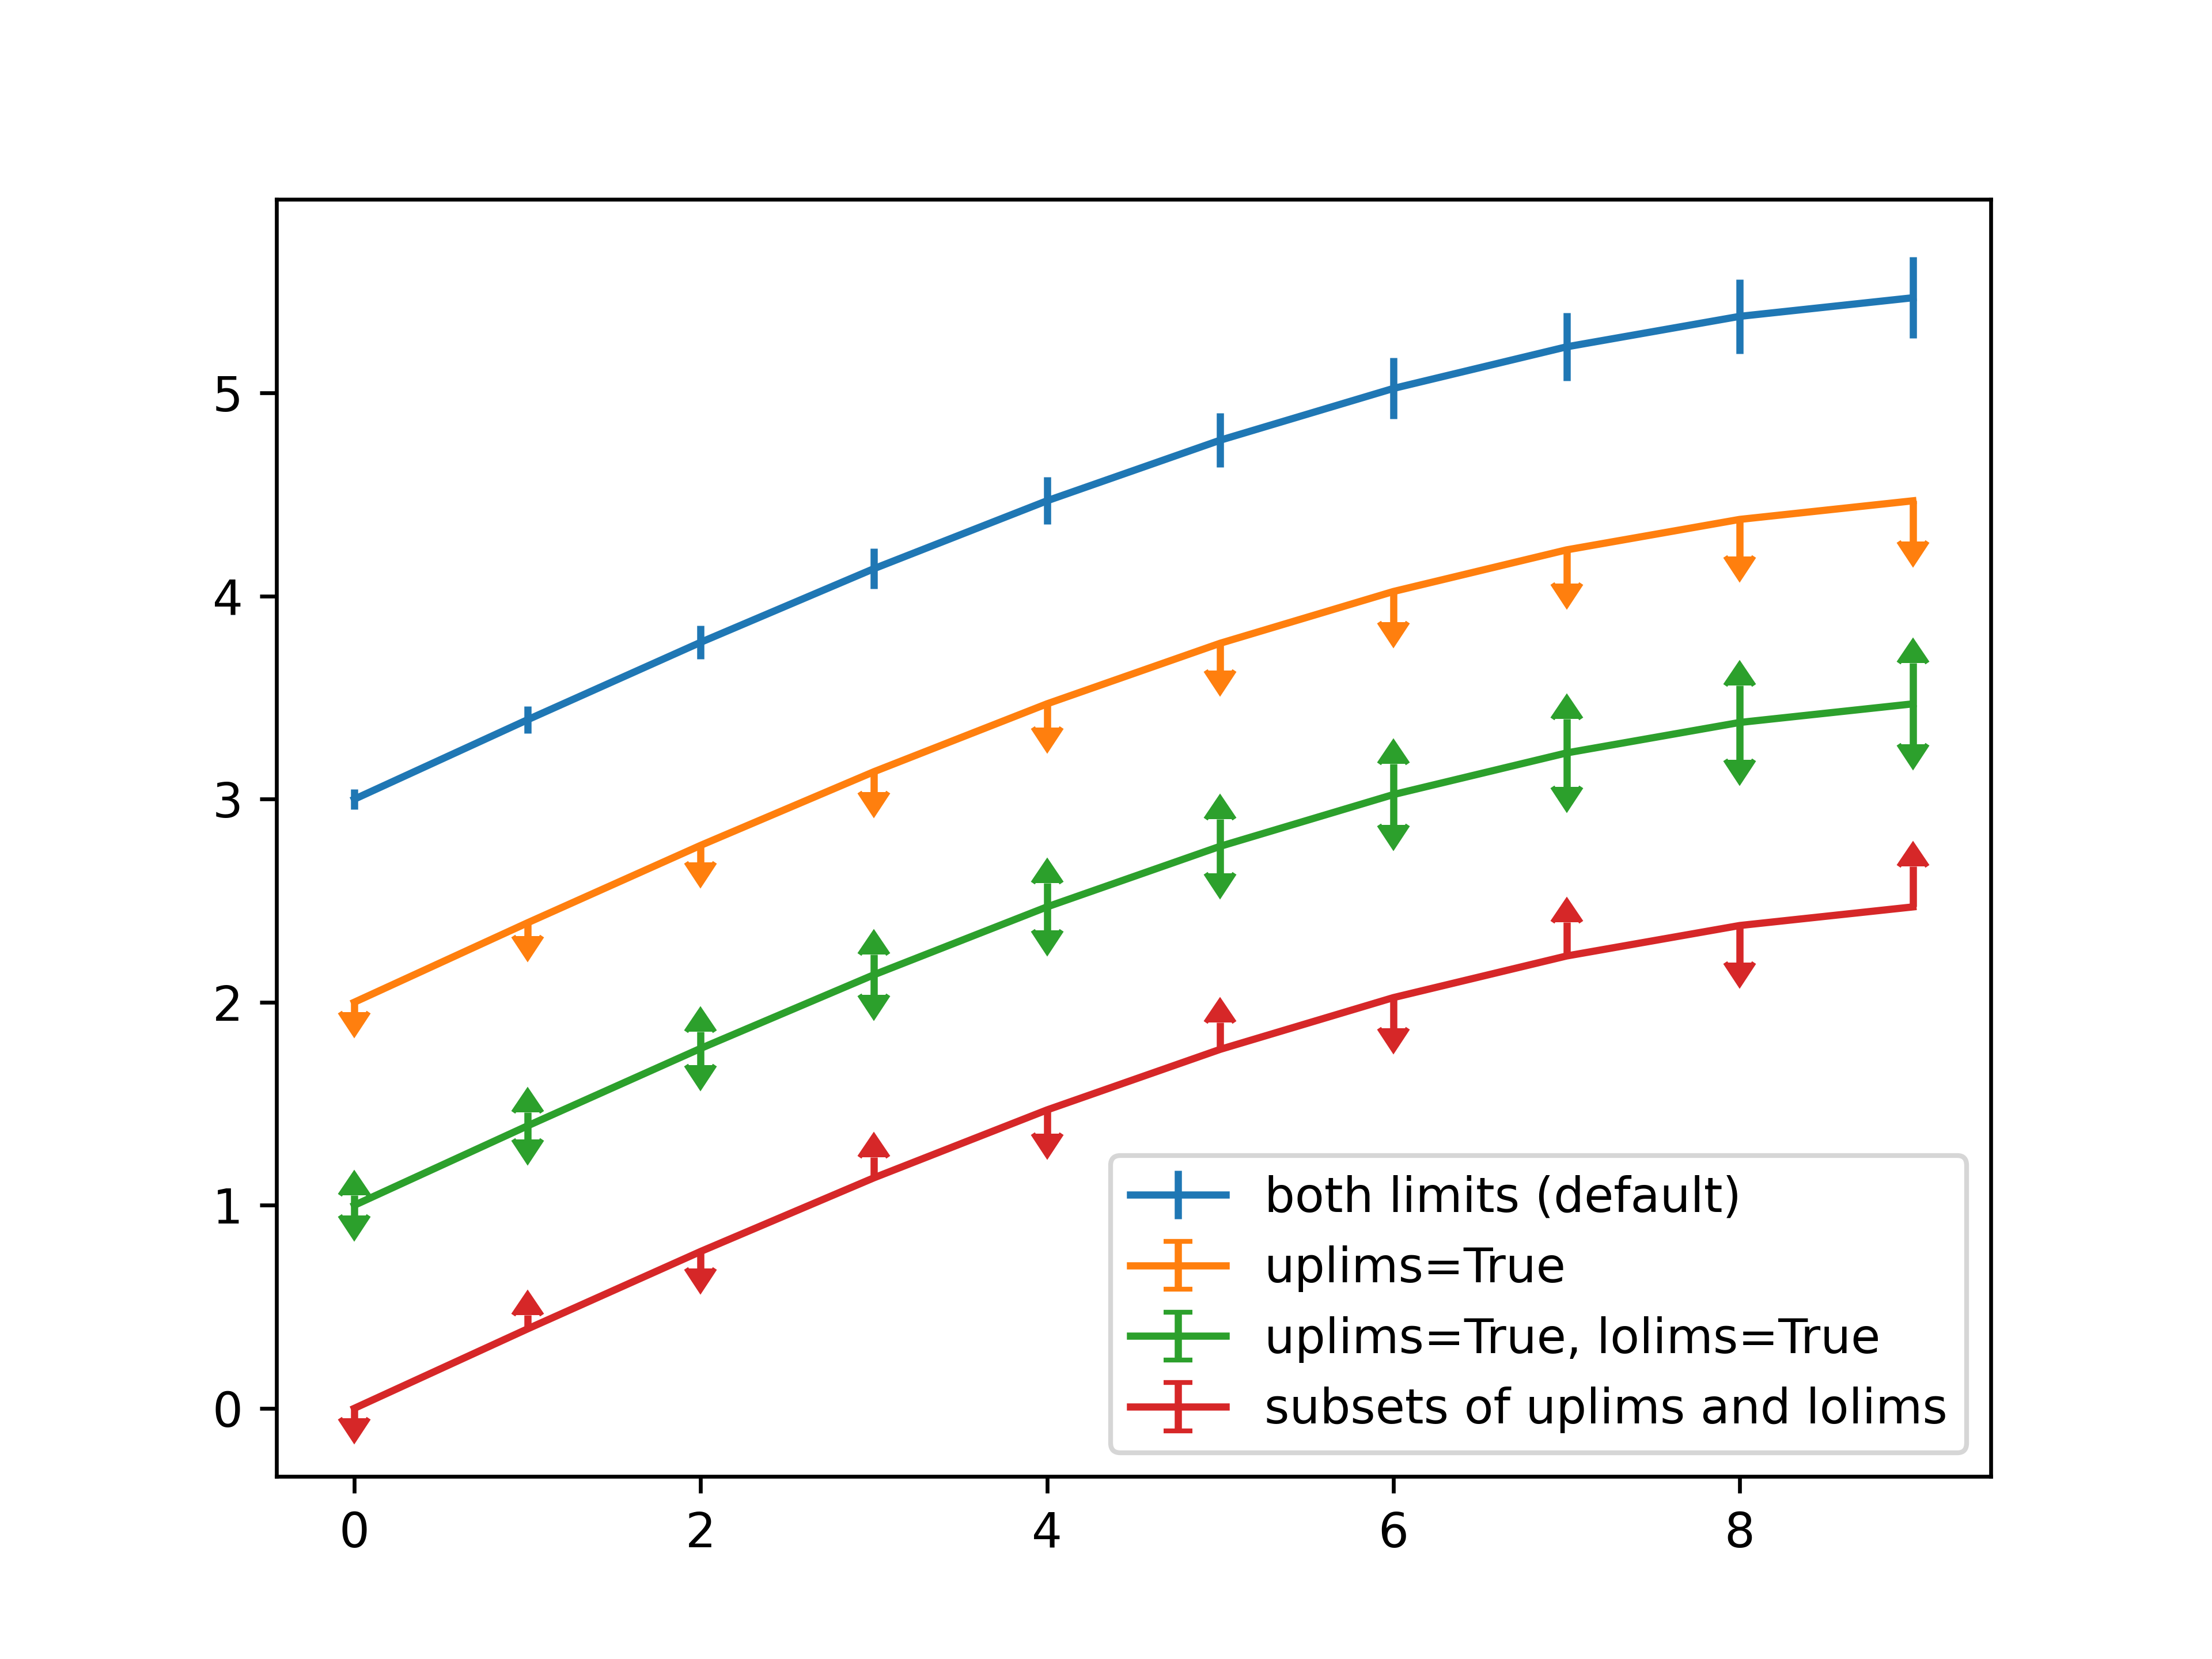
\includegraphics[width=0.6 \textwidth]{figs/chapter9/lines/UpLowErrorBar}
\caption{竖直方向误差限制选择线}
\end{figure}
\lstinputlisting[
    style       =   Python,
    caption     =   {\bf XYErrorBar.py},
    label       =   {XYErrorBar.py}
]{code/lines/XYErrorBar.py}
\begin{figure}[H]
\centering
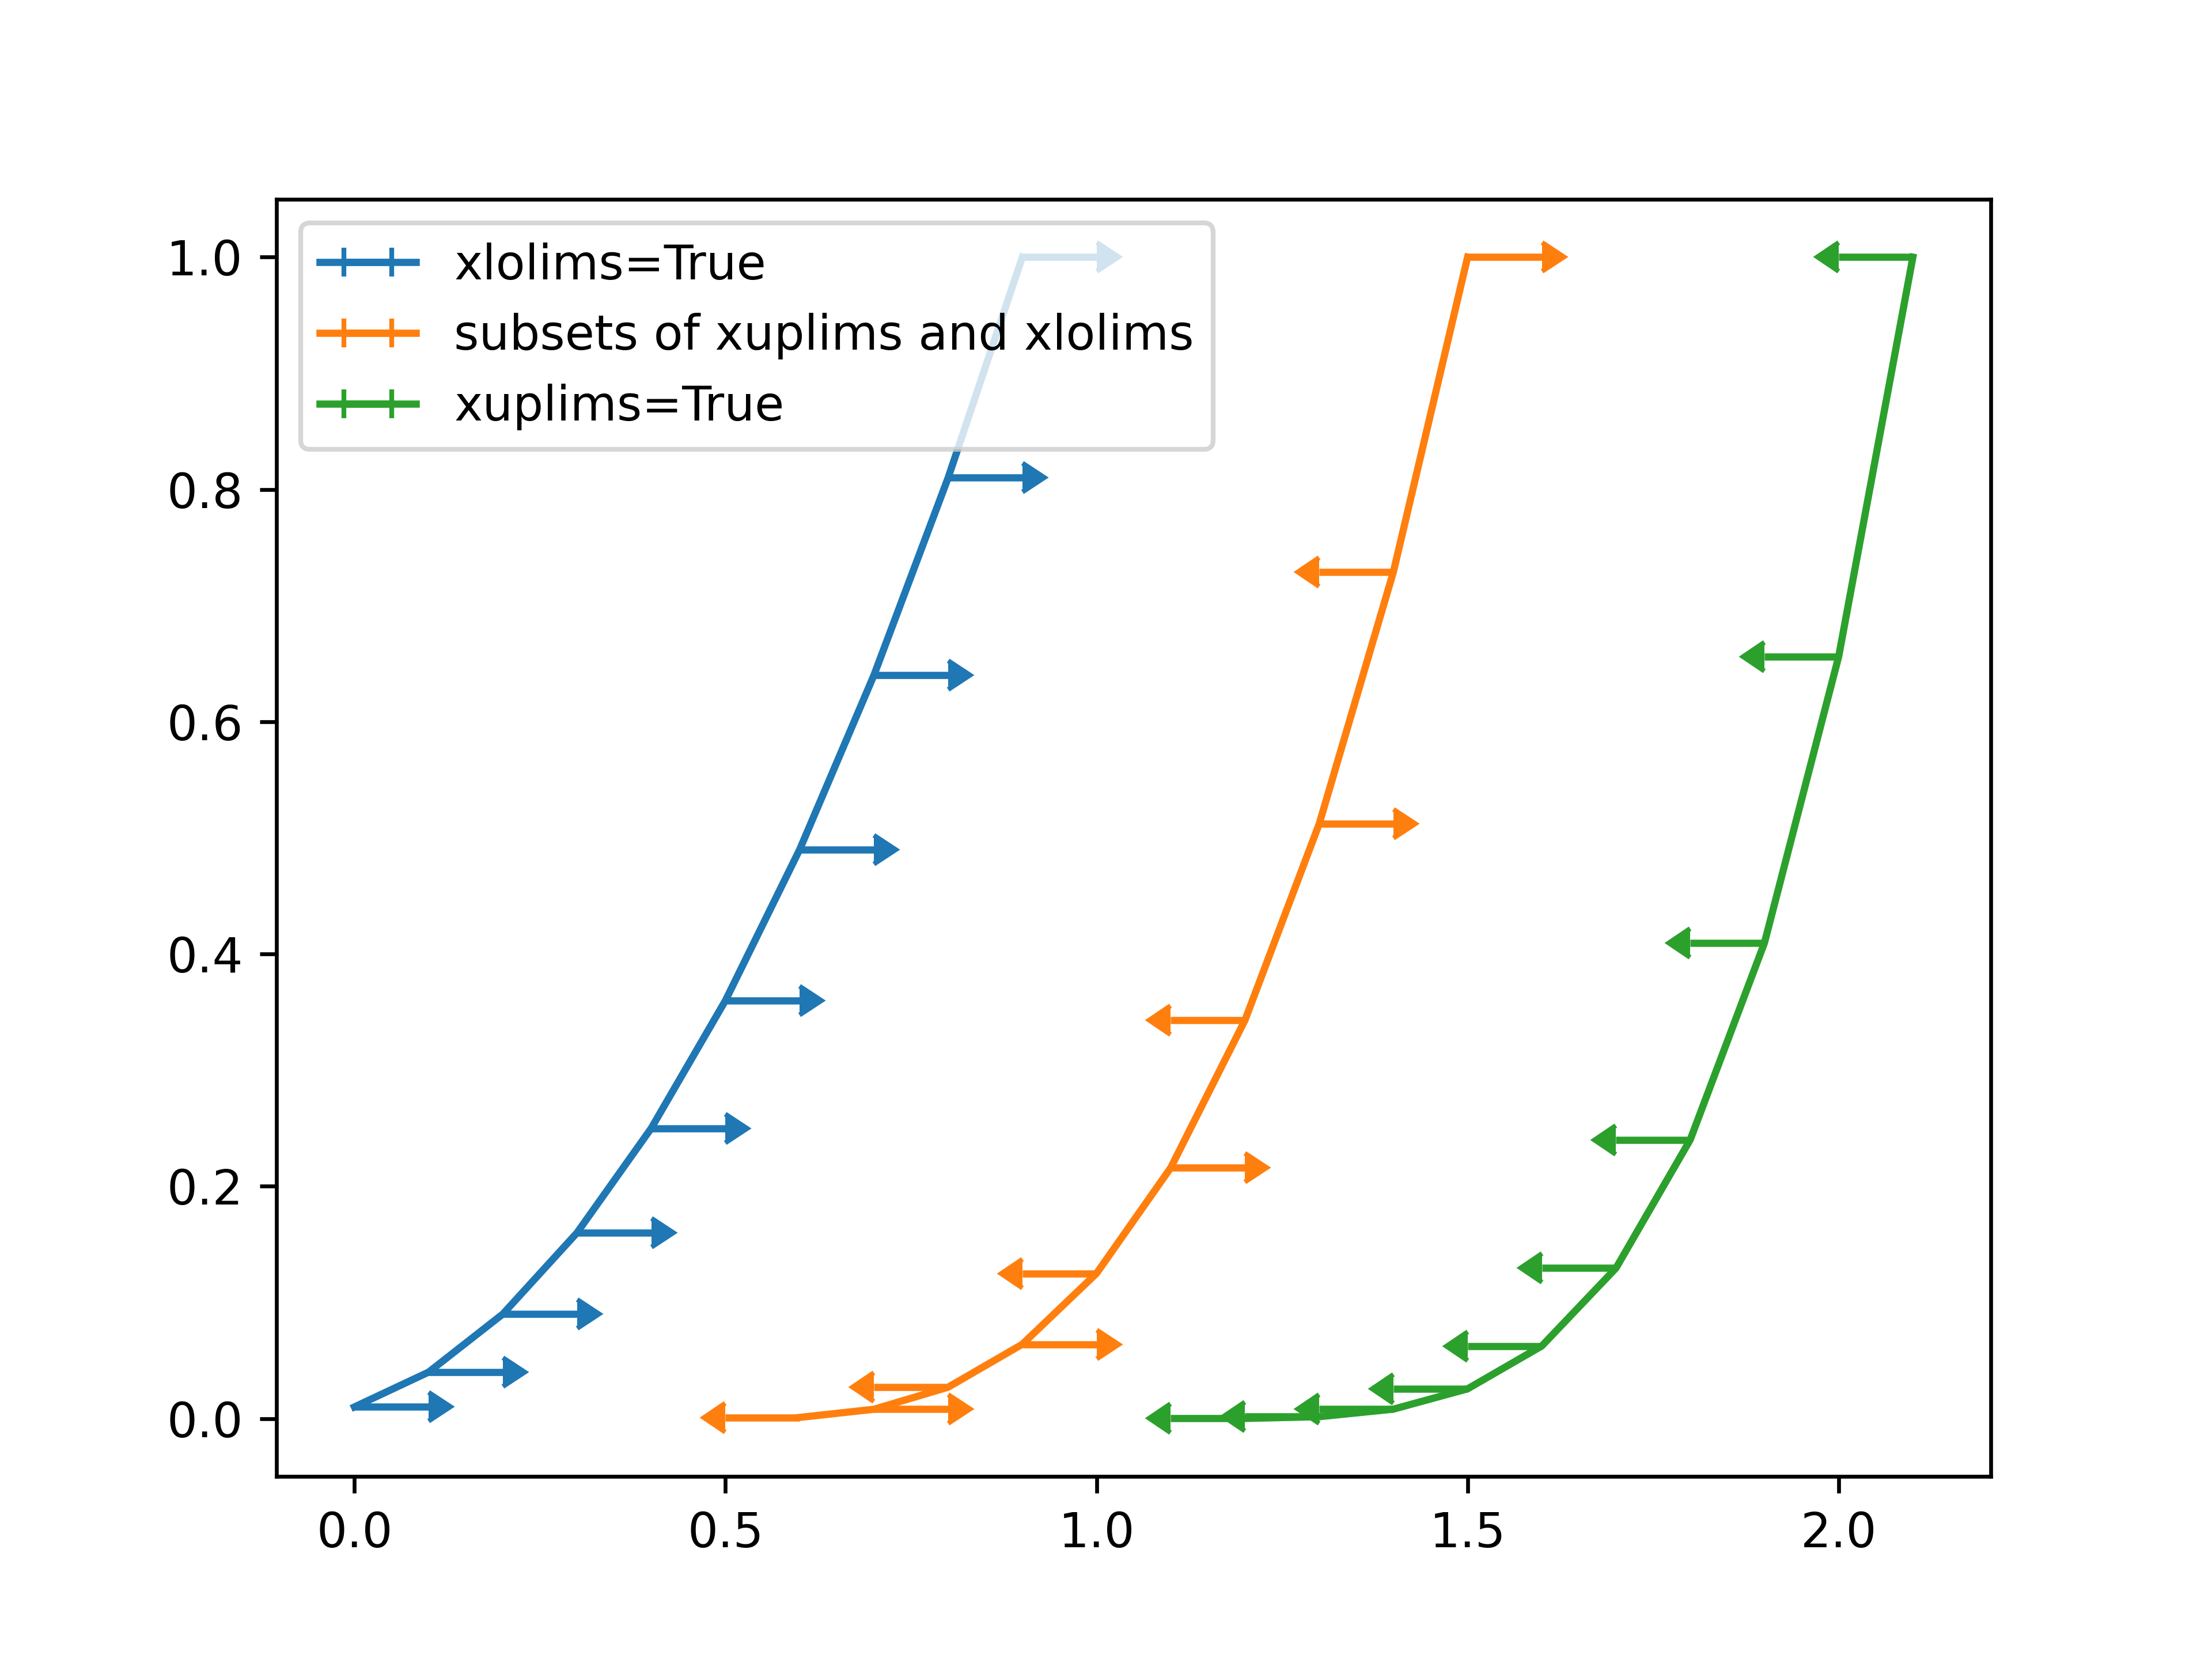
\includegraphics[width=0.6 \textwidth]{figs/chapter9/lines/XYErrorBar}
\caption{水平方向误差限制选择线}
\end{figure}

\subsection{误差带曲线}
\lstinputlisting[
    style       =   Python,
    caption     =   {\bf ErrorBandCurve.py},
    label       =   {ErrorBandCurve.py}
]{code/lines/ErrorBandCurve.py}
\begin{figure}[H]
\centering
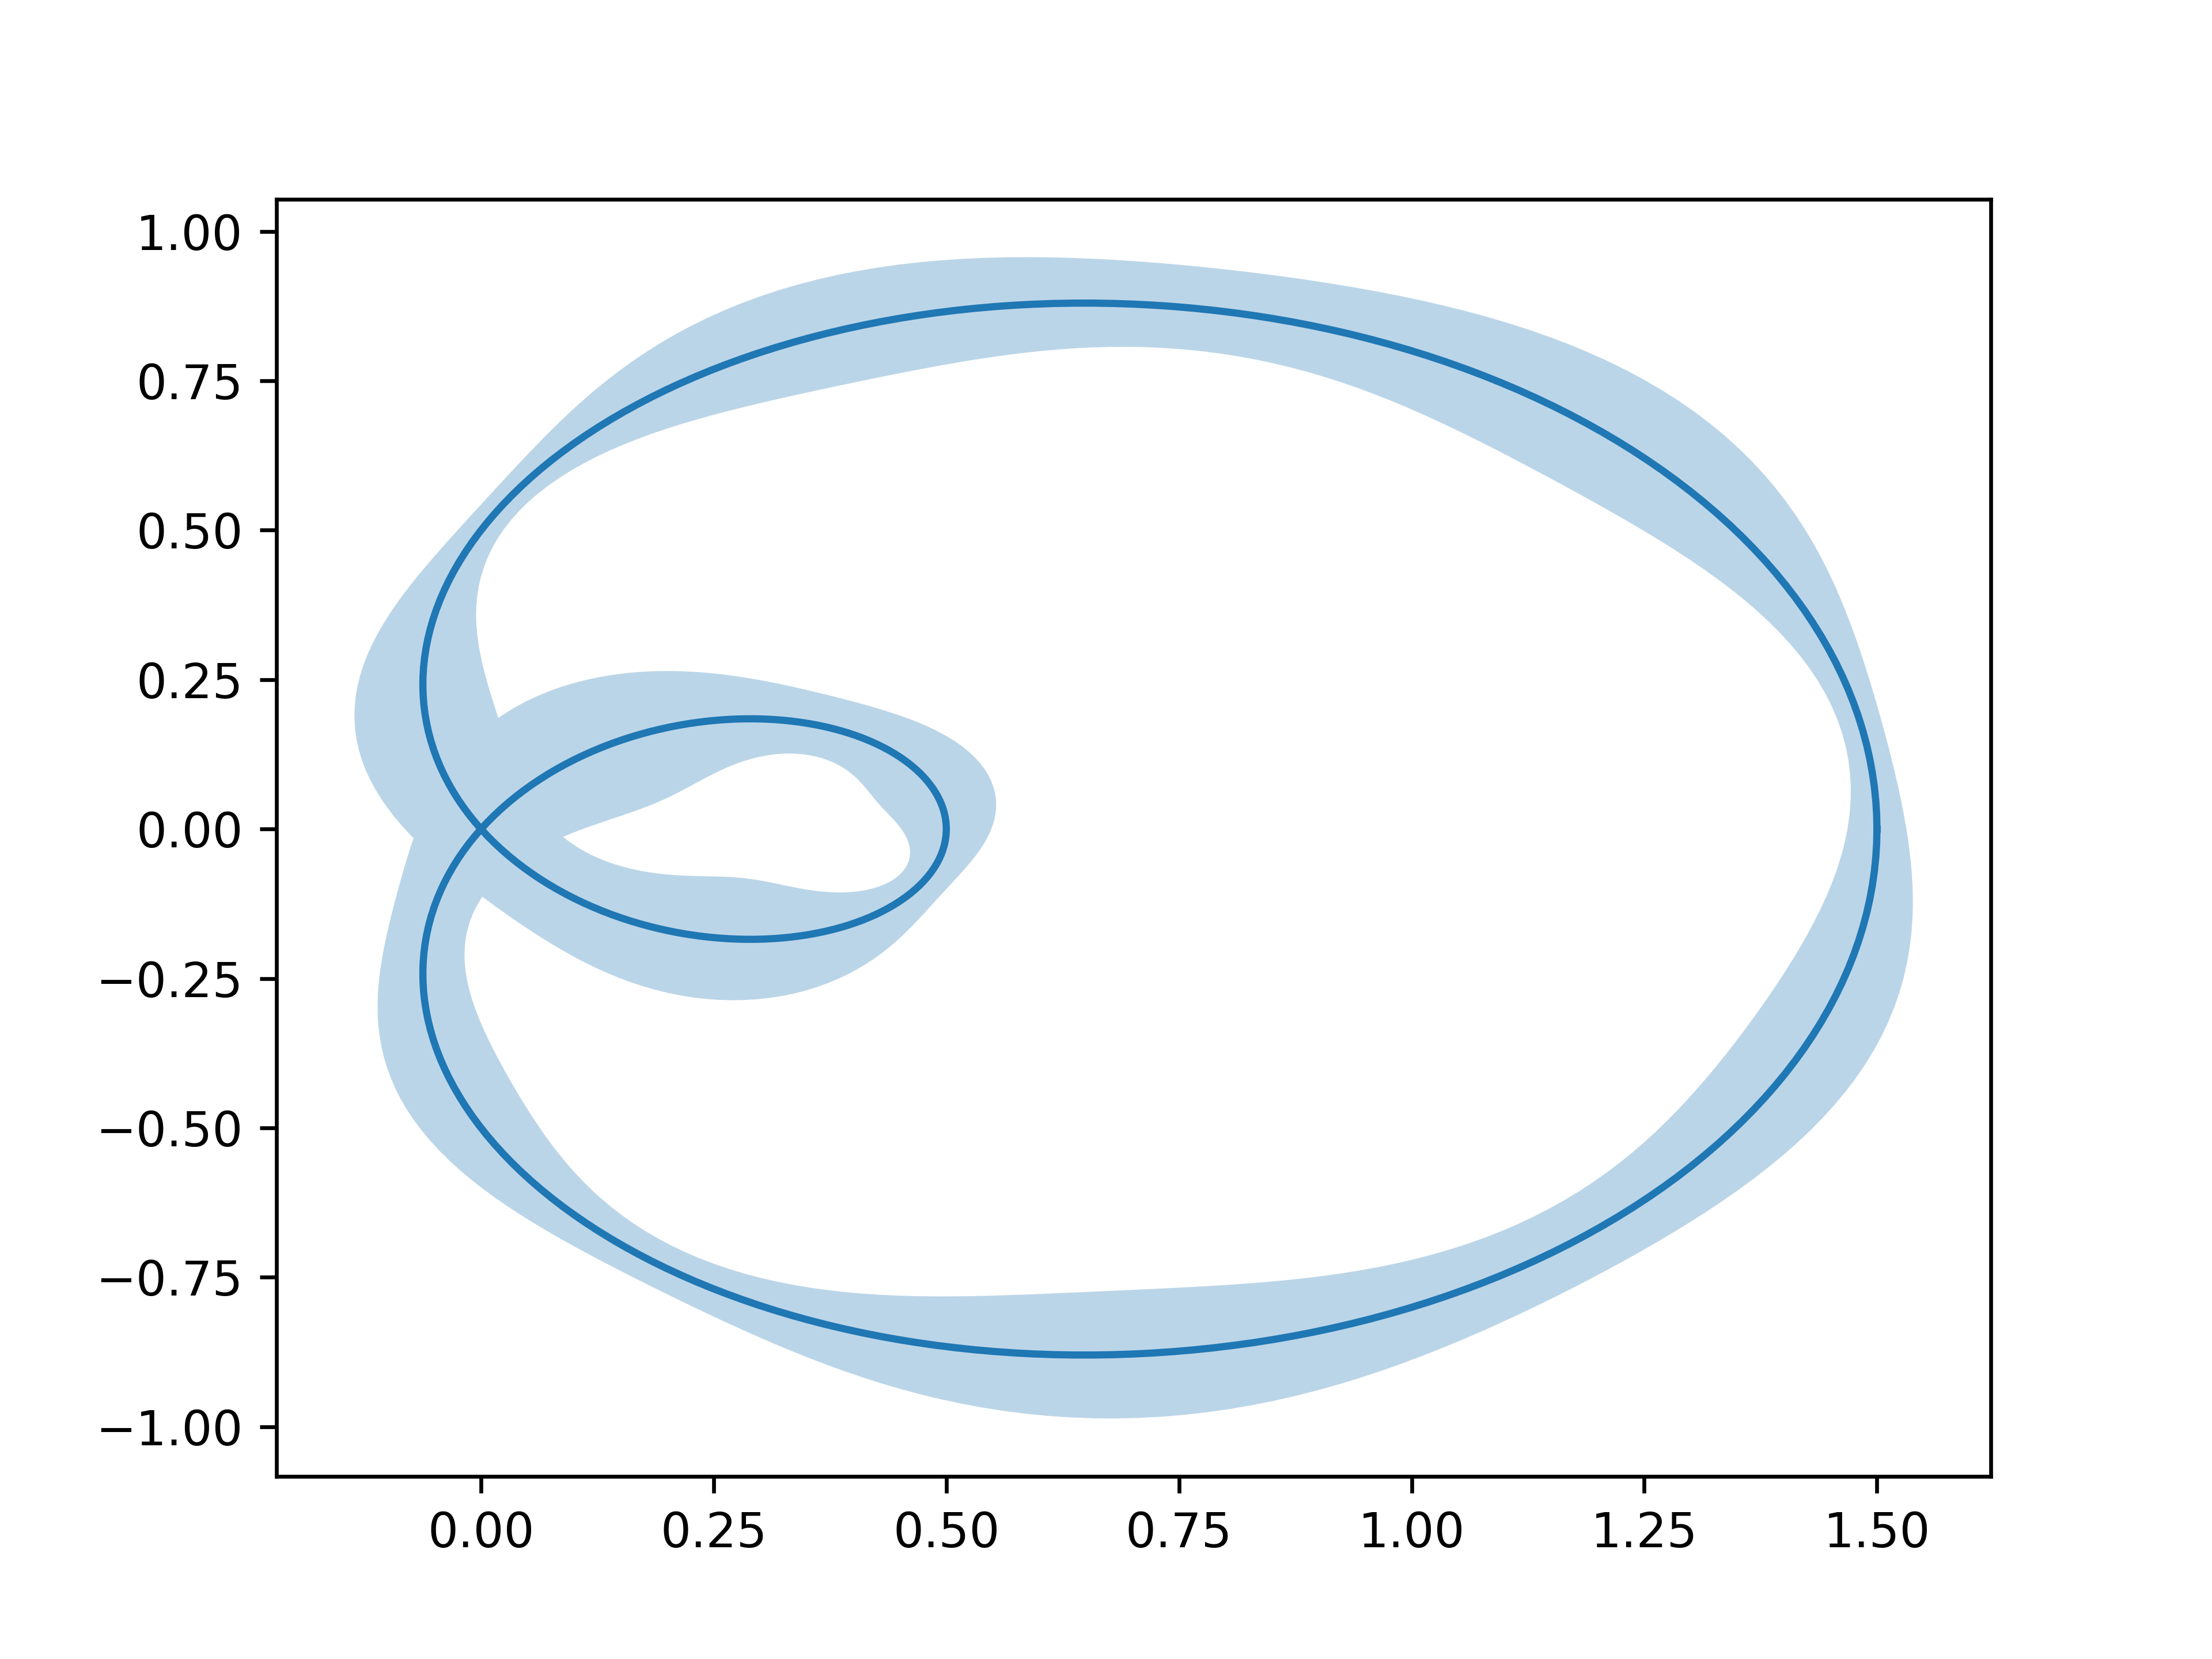
\includegraphics[width=0.6 \textwidth]{figs/chapter9/lines/ErrorBandCurve}
\caption{误差带曲线}
\end{figure}



\section{柱状图}
\subsection{简单的柱状图}
\lstinputlisting[
    style       =   Python,
    caption     =   {\bf SimpleBar.py},
    label       =   {SimpleBar.py}
]{code/bars/SimpleBar.py}
\begin{figure}[H]
\centering
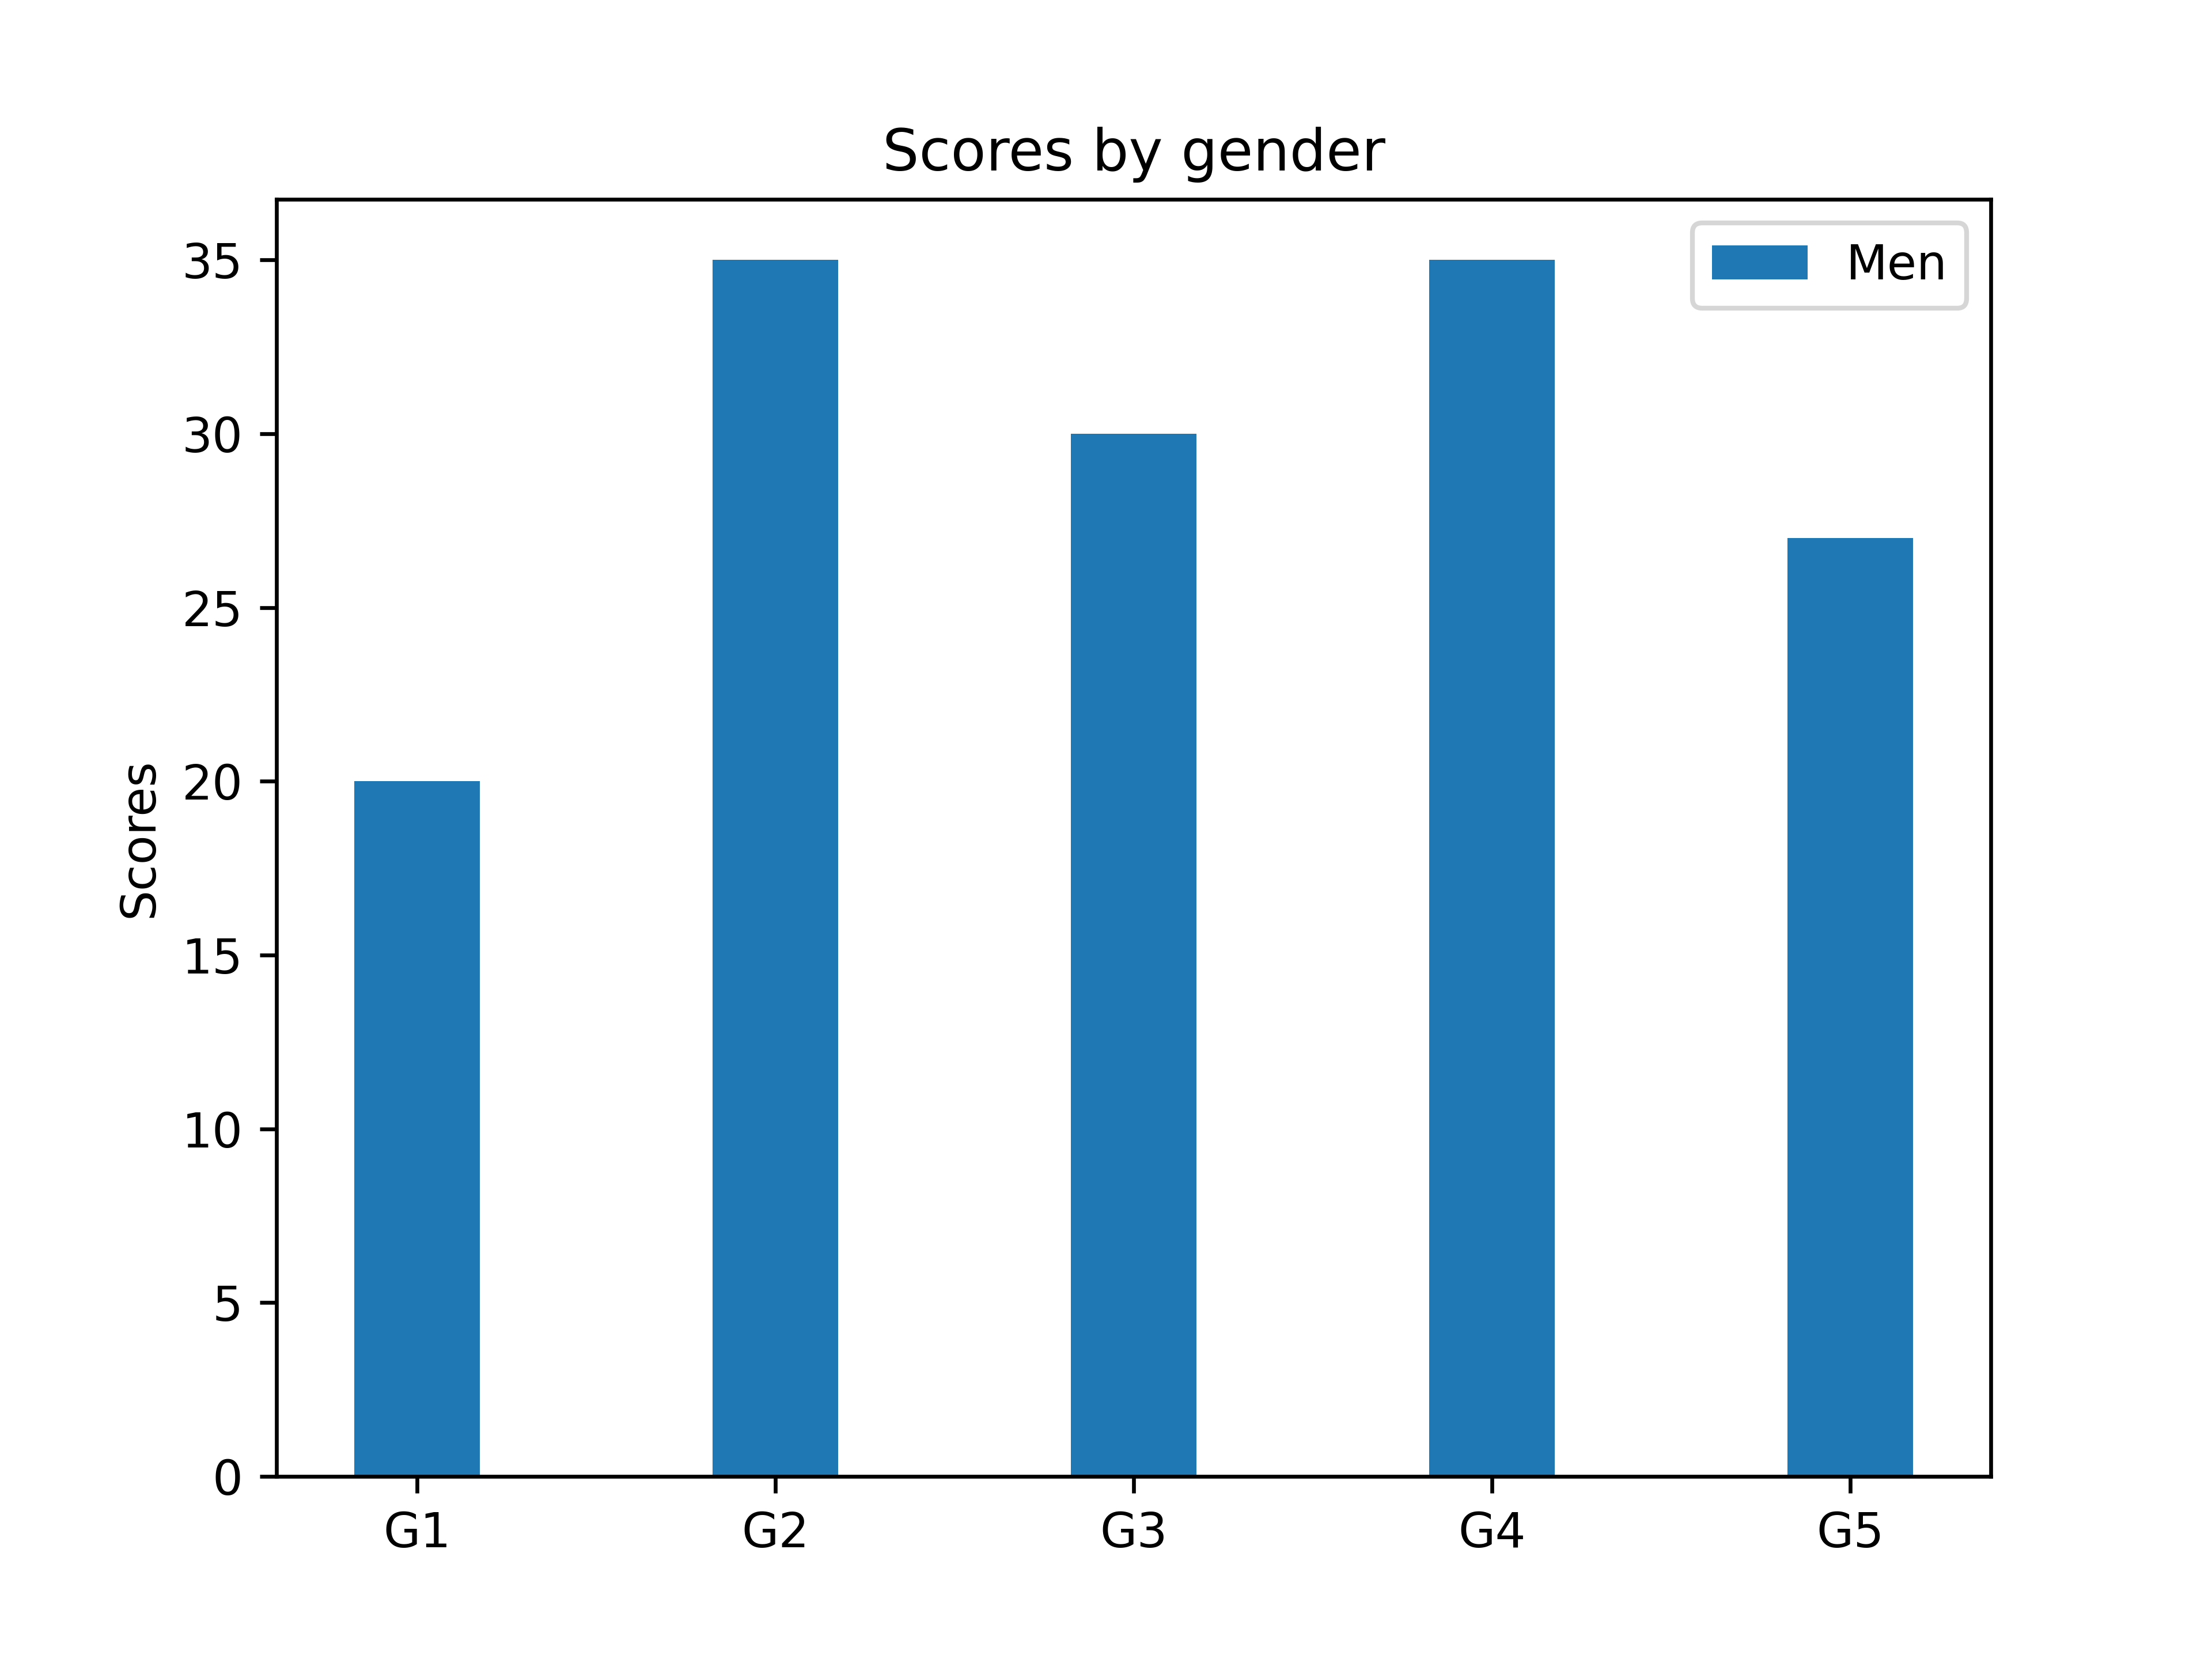
\includegraphics[width=0.6 \textwidth]{figs/chapter9/bars/SimpleBar}
\caption{简单的柱状图}
\end{figure}

\subsection{水平条形图}
\lstinputlisting[
    style       =   Python,
    caption     =   {\bf HorizontalBar.py},
    label       =   {HorizontalBar.py}
]{code/bars/HorizontalBar.py}
\begin{figure}[H]
\centering
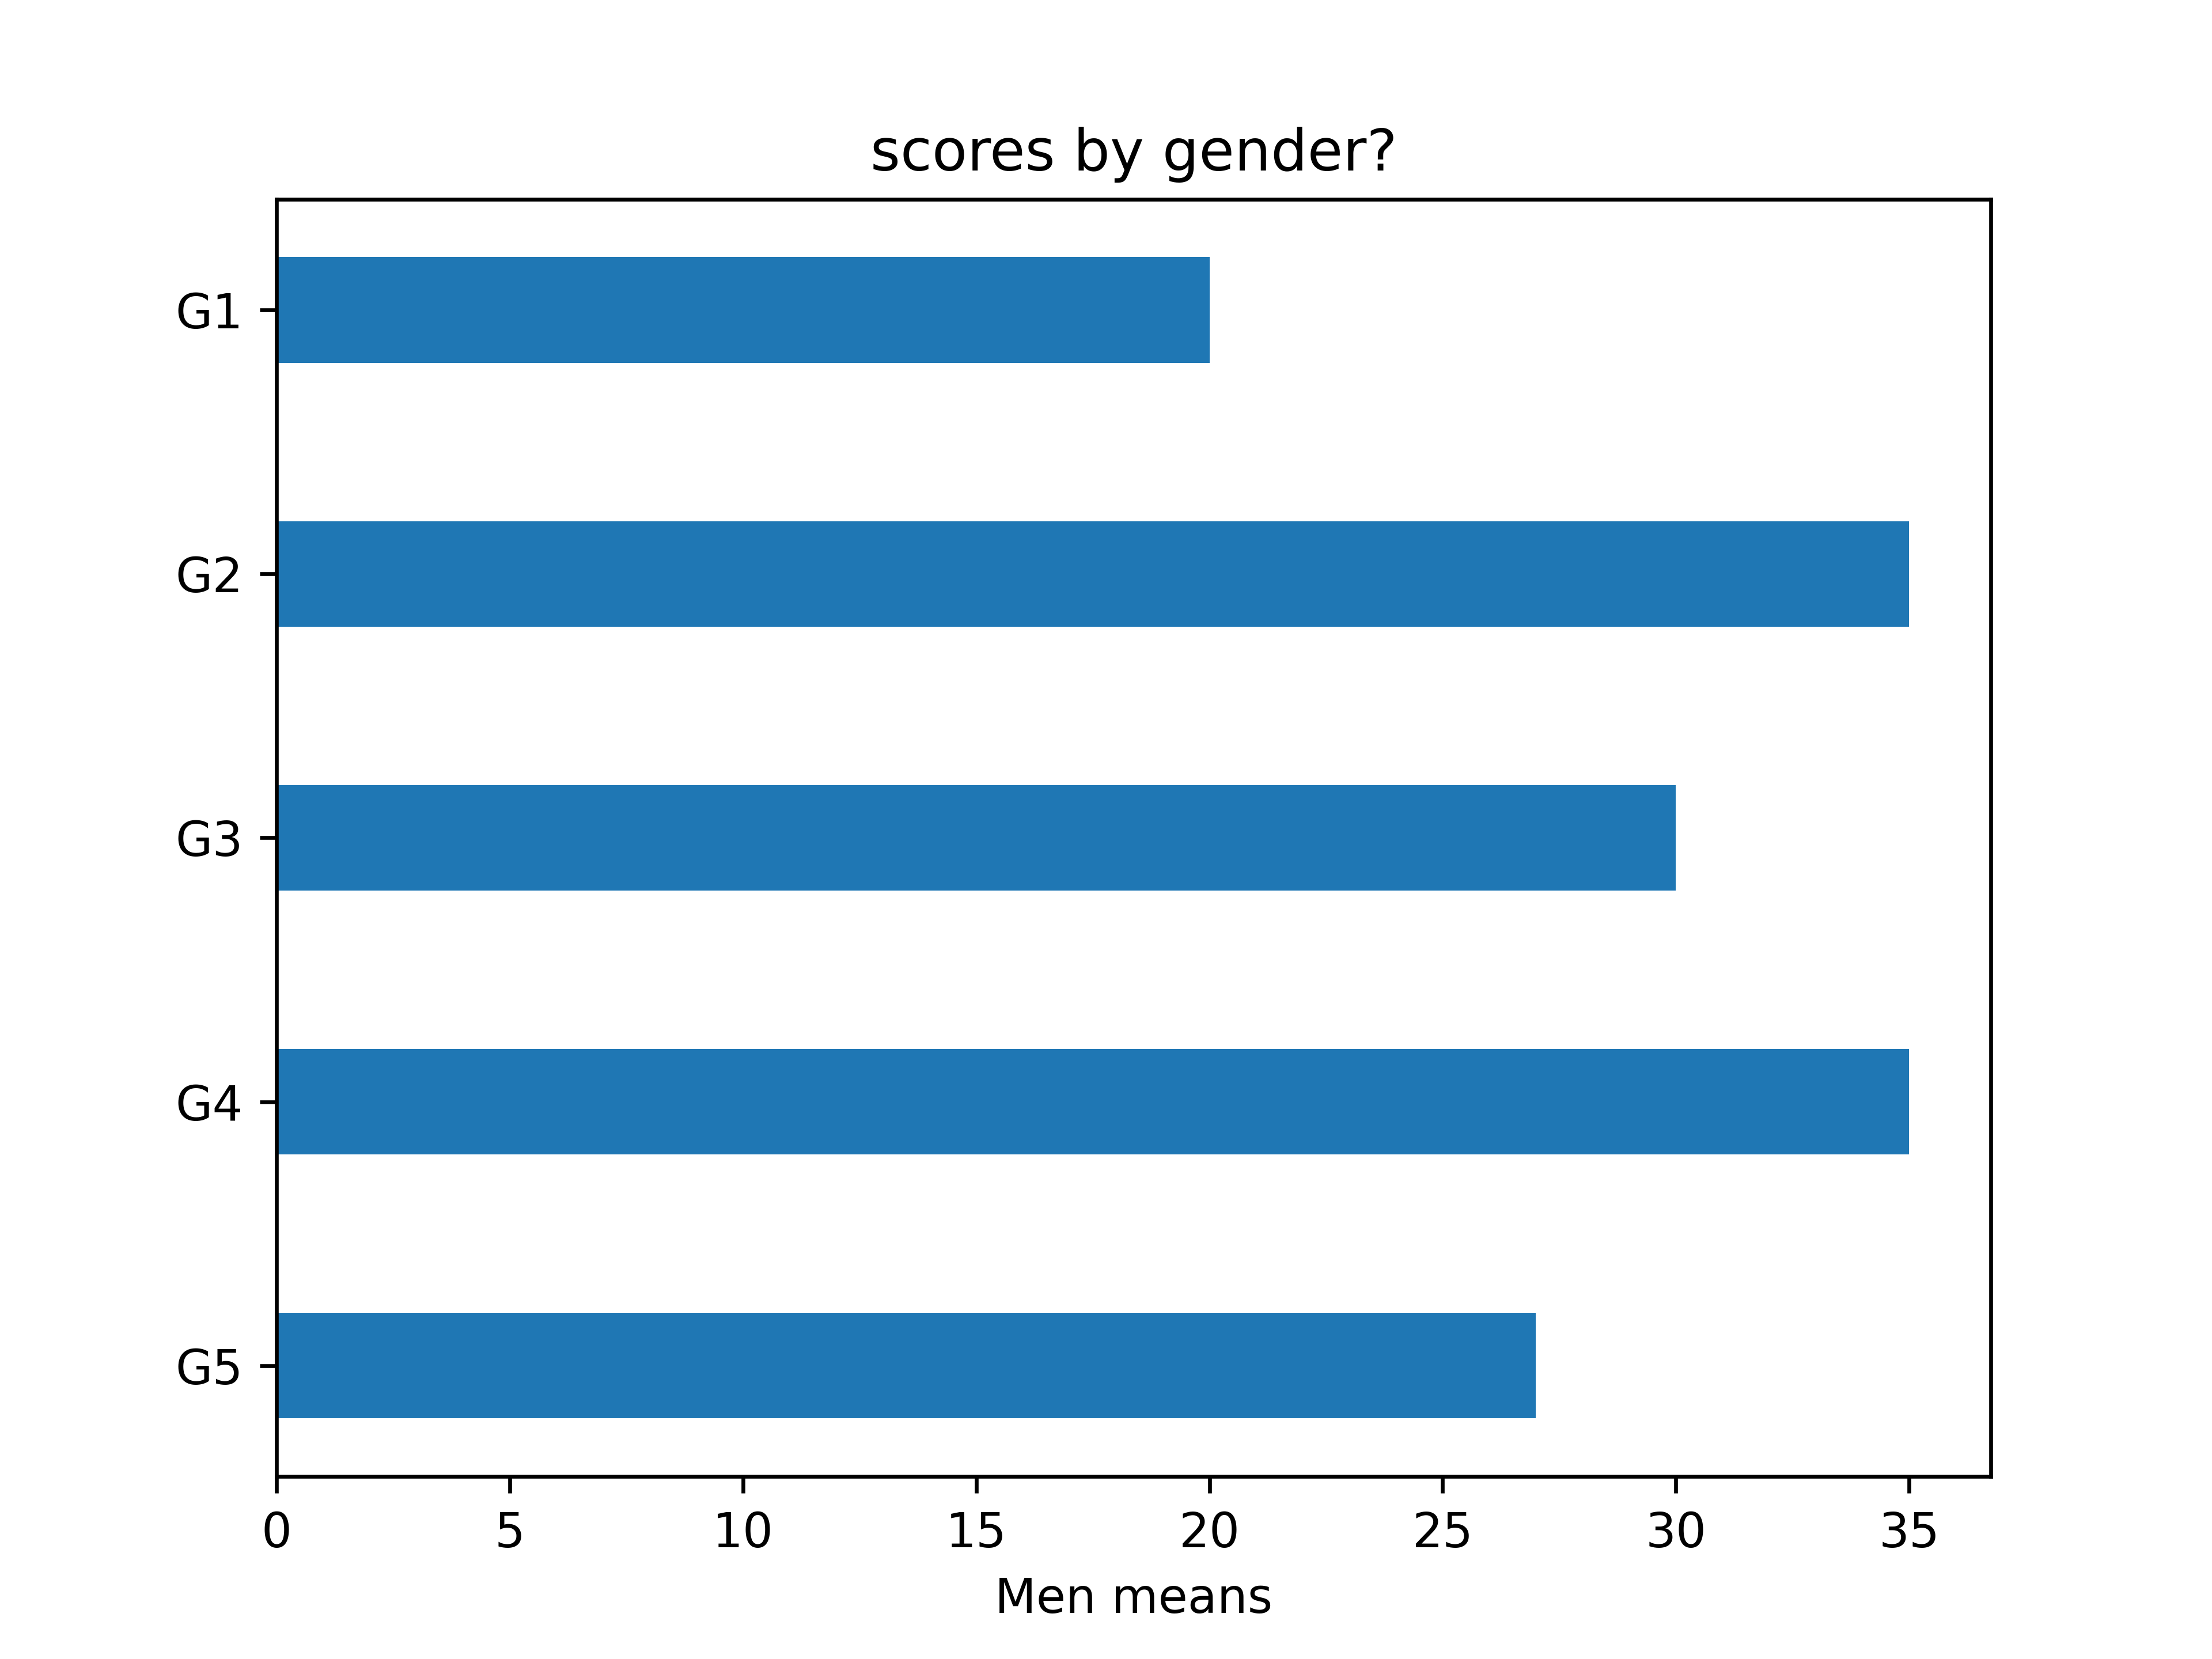
\includegraphics[width=0.6 \textwidth]{figs/chapter9/bars/HorizontalBar}
\caption{水平条形图}
\end{figure}

\subsection{带有误差线的柱状图}
\lstinputlisting[
    style       =   Python,
    caption     =   {\bf StackedBar.py},
    label       =   {StackedBar.py}
]{code/bars/StackedBar.py}
\begin{figure}[H]
\centering
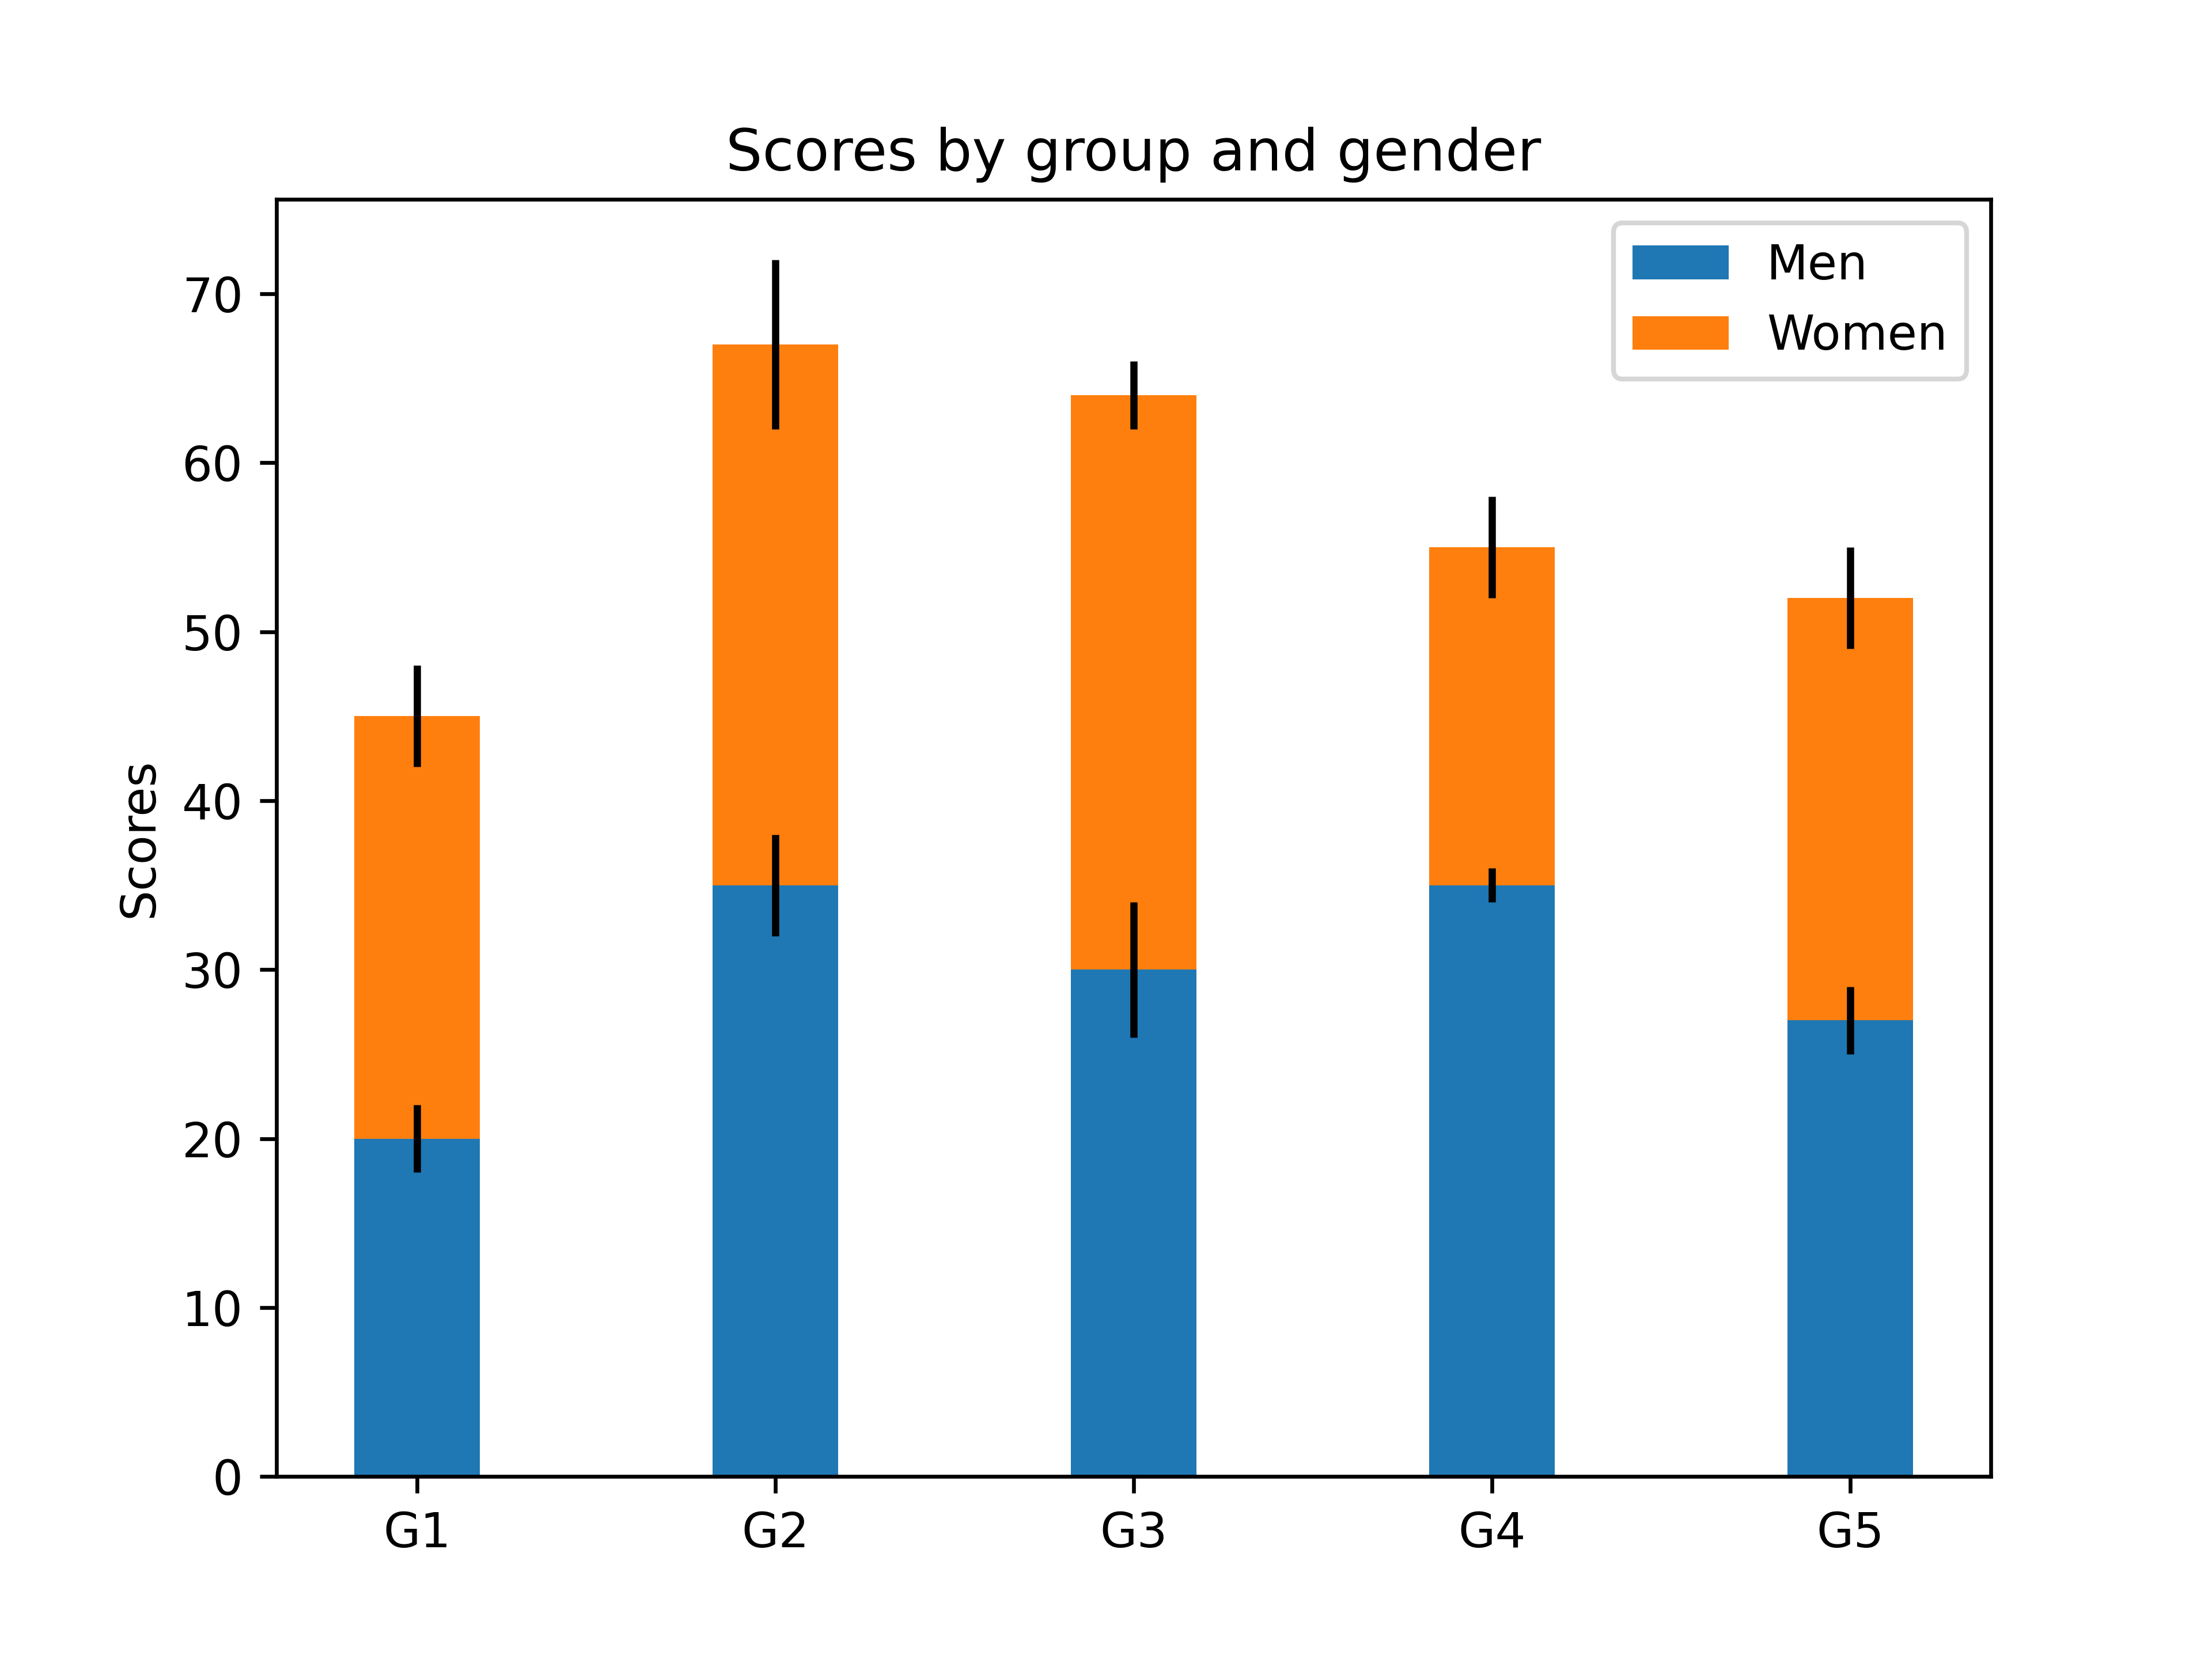
\includegraphics[width=0.6 \textwidth]{figs/chapter9/bars/StackedBar}
\caption{带误差线的堆叠柱状图}
\end{figure}

\subsection{带标签的分组柱状图}
\lstinputlisting[
    style       =   Python,
    caption     =   {\bf GroupedBar.py},
    label       =   {GroupedBar.py}
]{code/bars/GroupedBar.py}
\begin{figure}[H]
\centering
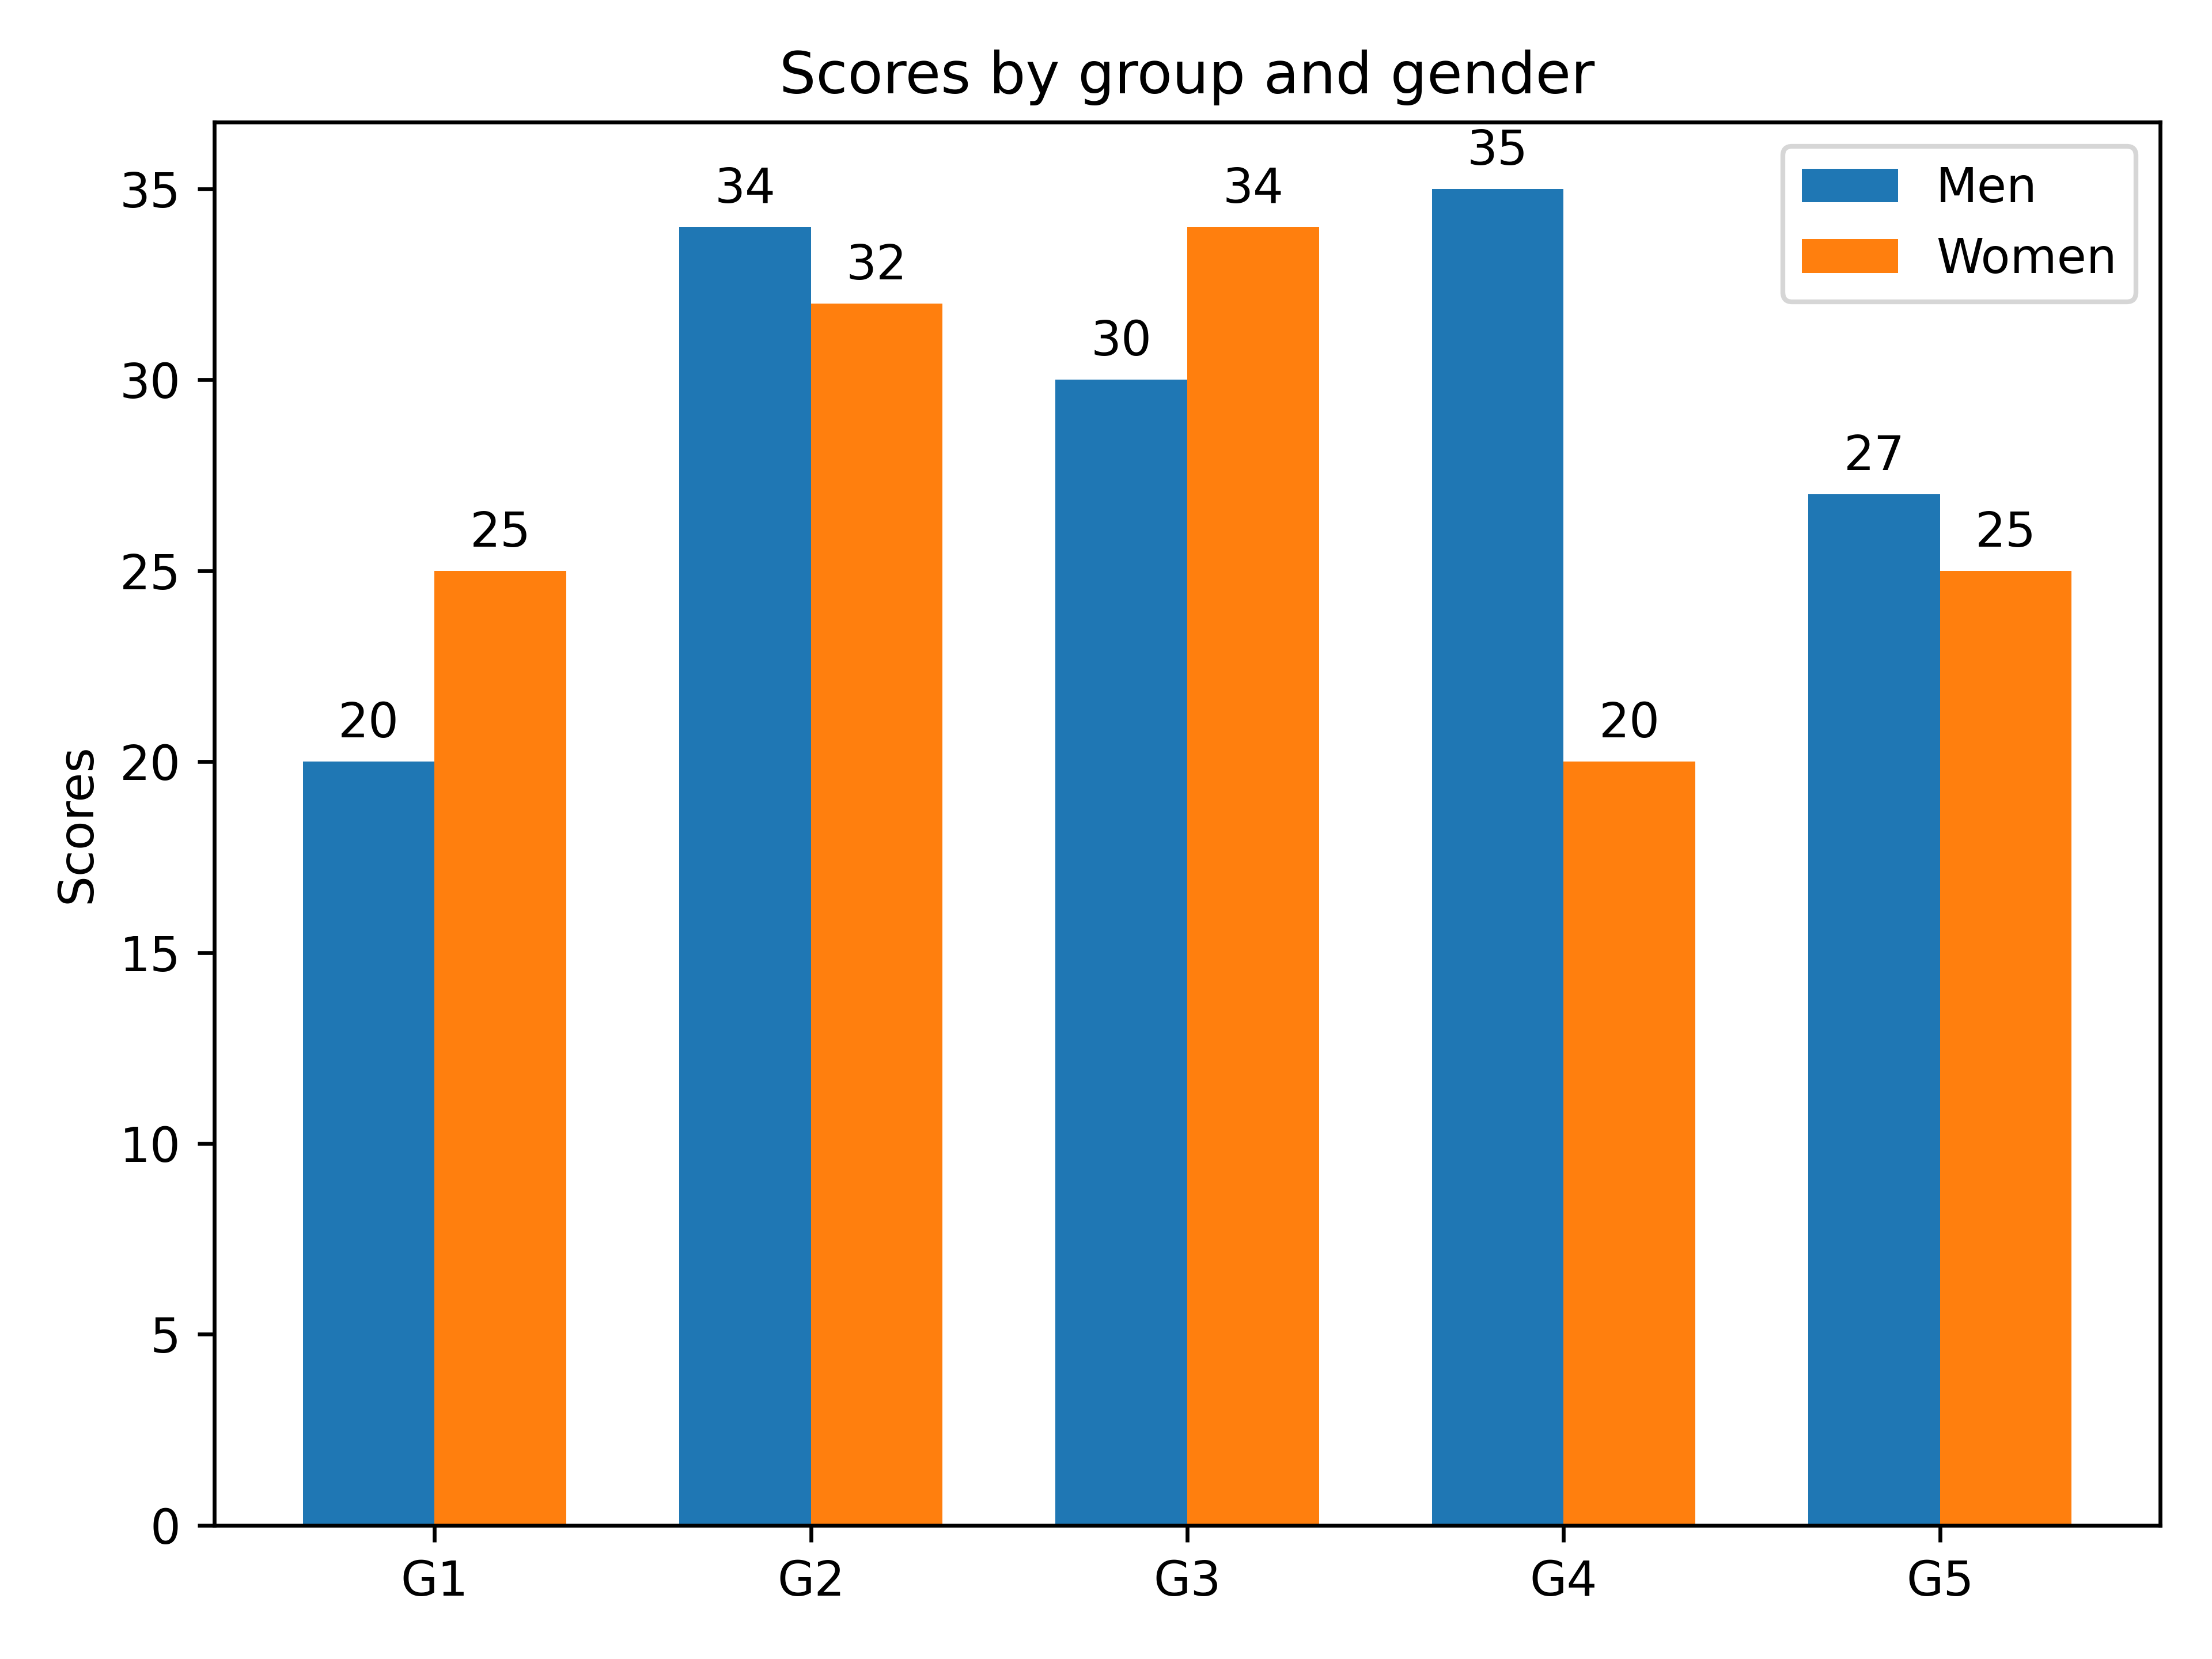
\includegraphics[width=0.6 \textwidth]{figs/chapter9/bars/GroupedBar}
\caption{带标签的分组柱状图}
\end{figure}

\subsection{离散分布条形图}
\lstinputlisting[
    style       =   Python,
    caption     =   {\bf DiscreteDistributionBar.py},
    label       =   {DiscreteDistributionBar.py}
]{code/bars/DiscreteDistributionBar.py}
\begin{figure}[H]
\centering
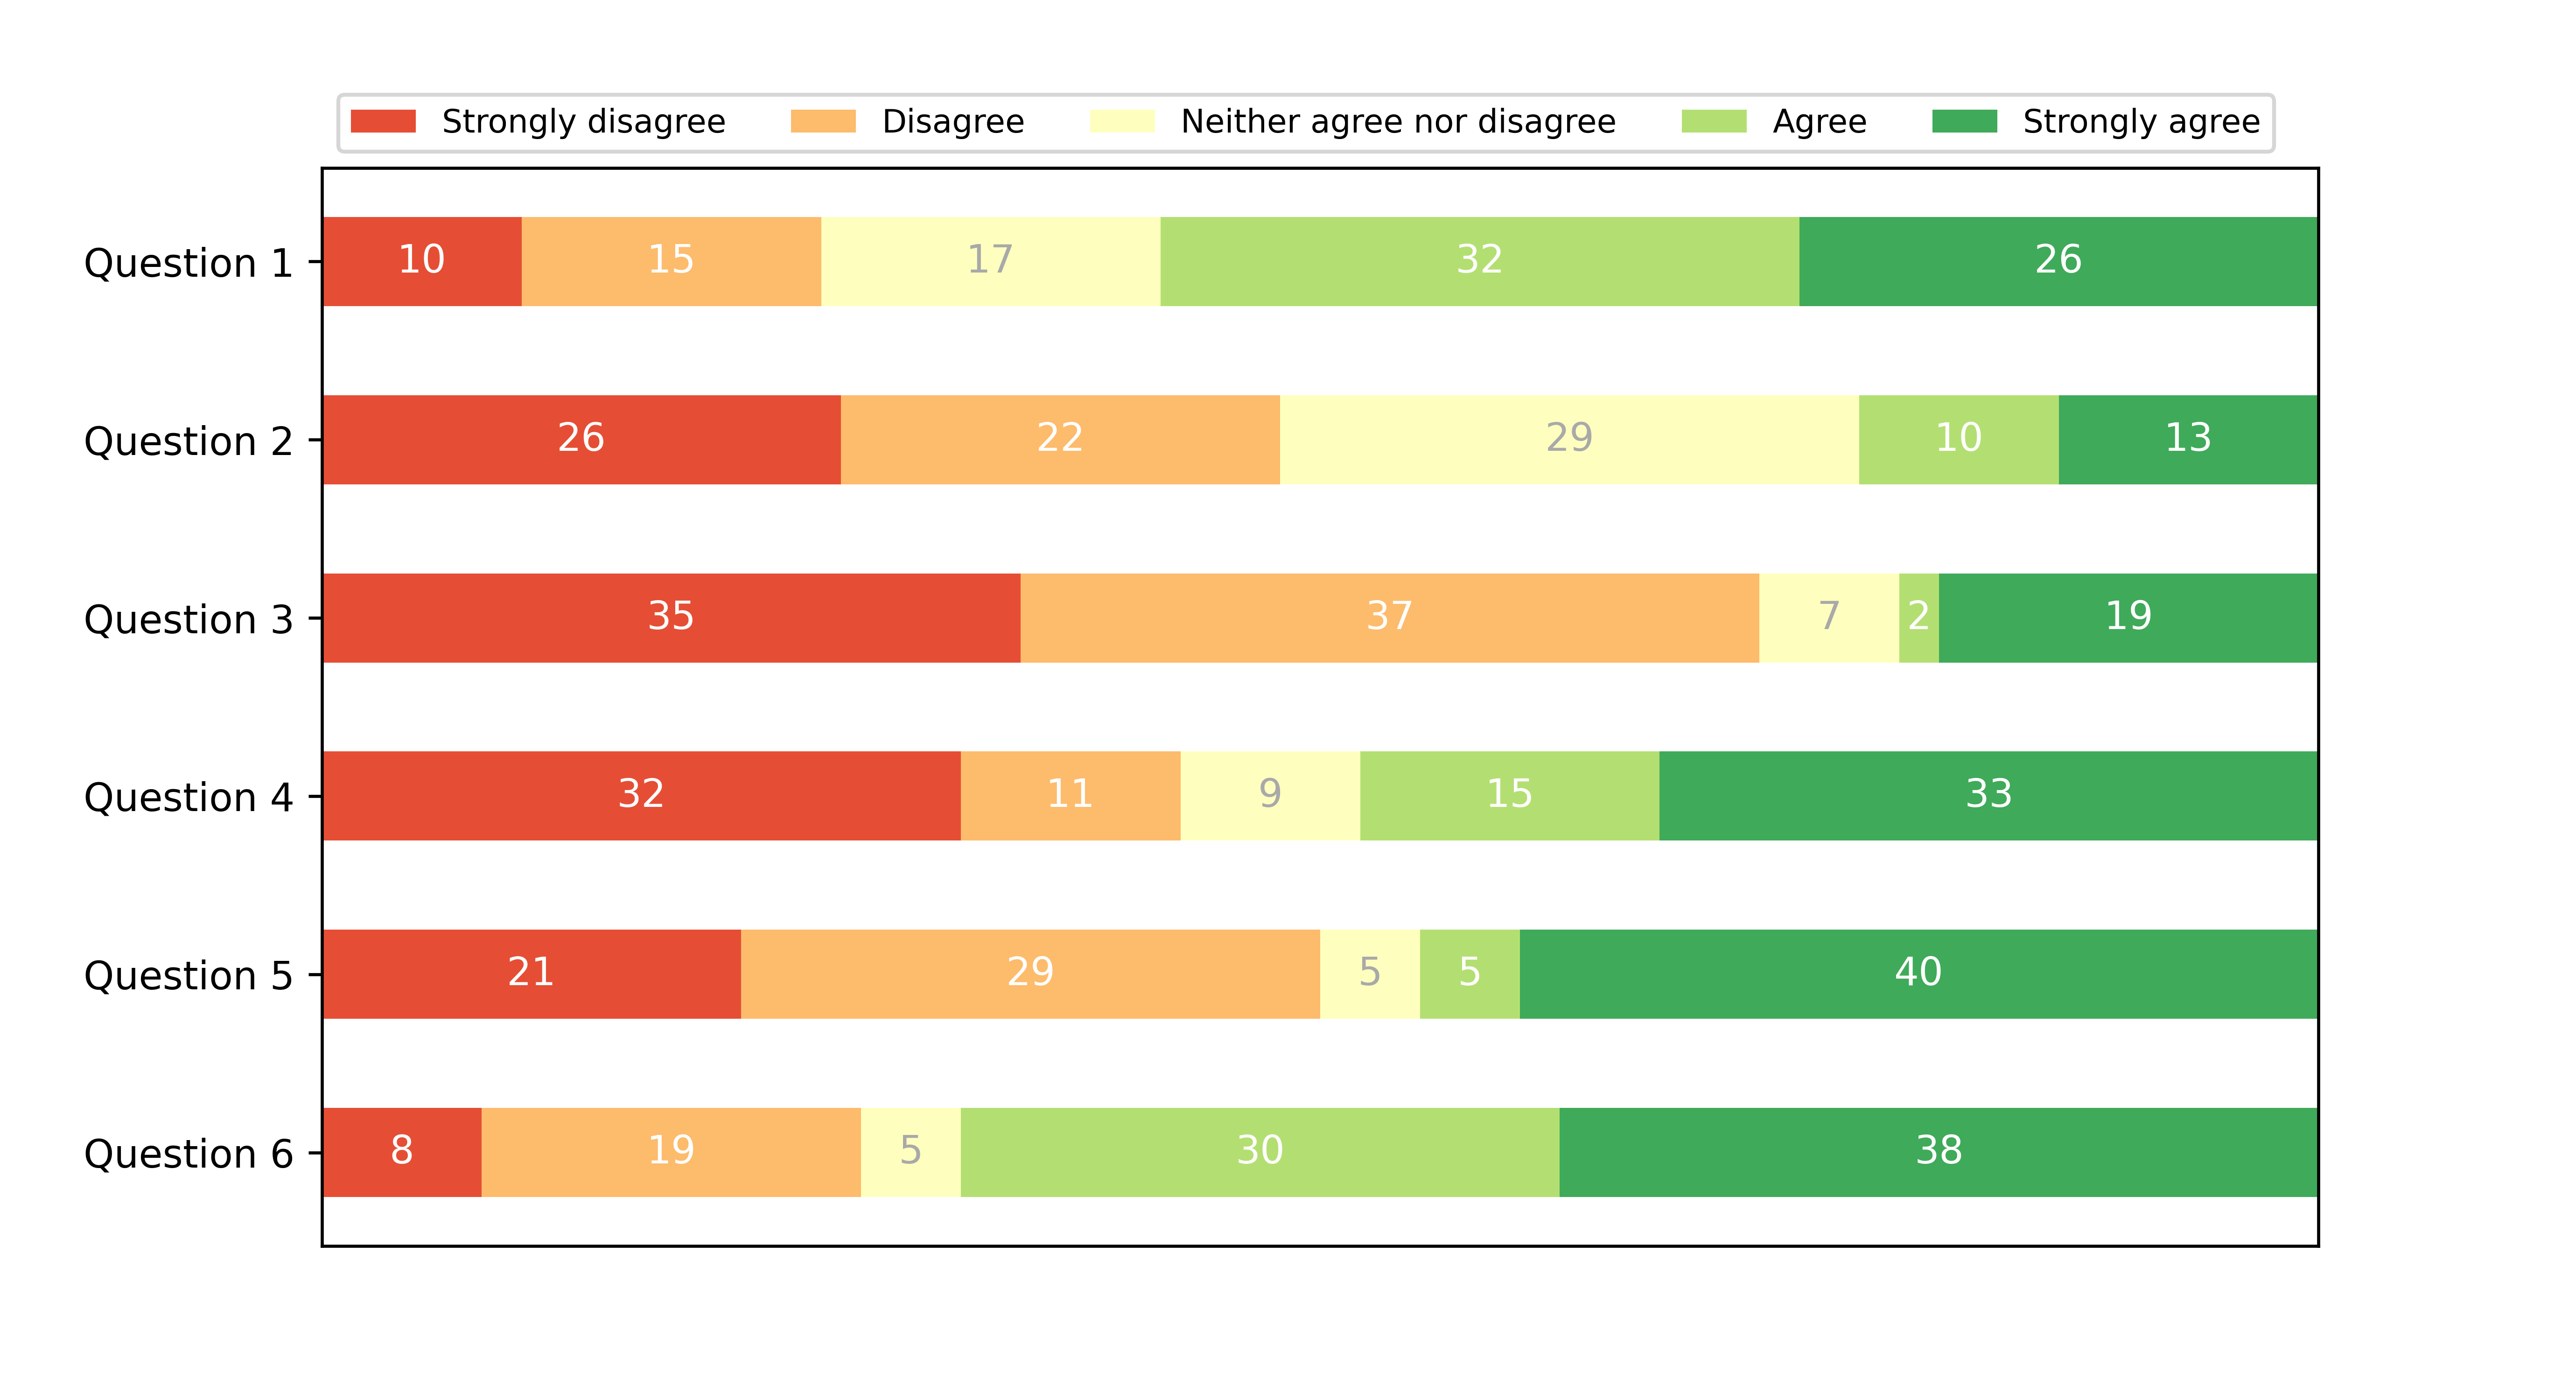
\includegraphics[width=0.6 \textwidth]{figs/chapter9/bars/DiscreteDistributionBar}
\caption{离散分布条形图}
\end{figure}
\subsection{破碎的条形图}
\lstinputlisting[
    style       =   Python,
    caption     =   {\bf BrokenBar.py},
    label       =   {BrokenBar.py}
]{code/bars/BrokenBar.py}
\begin{figure}[H]
\centering
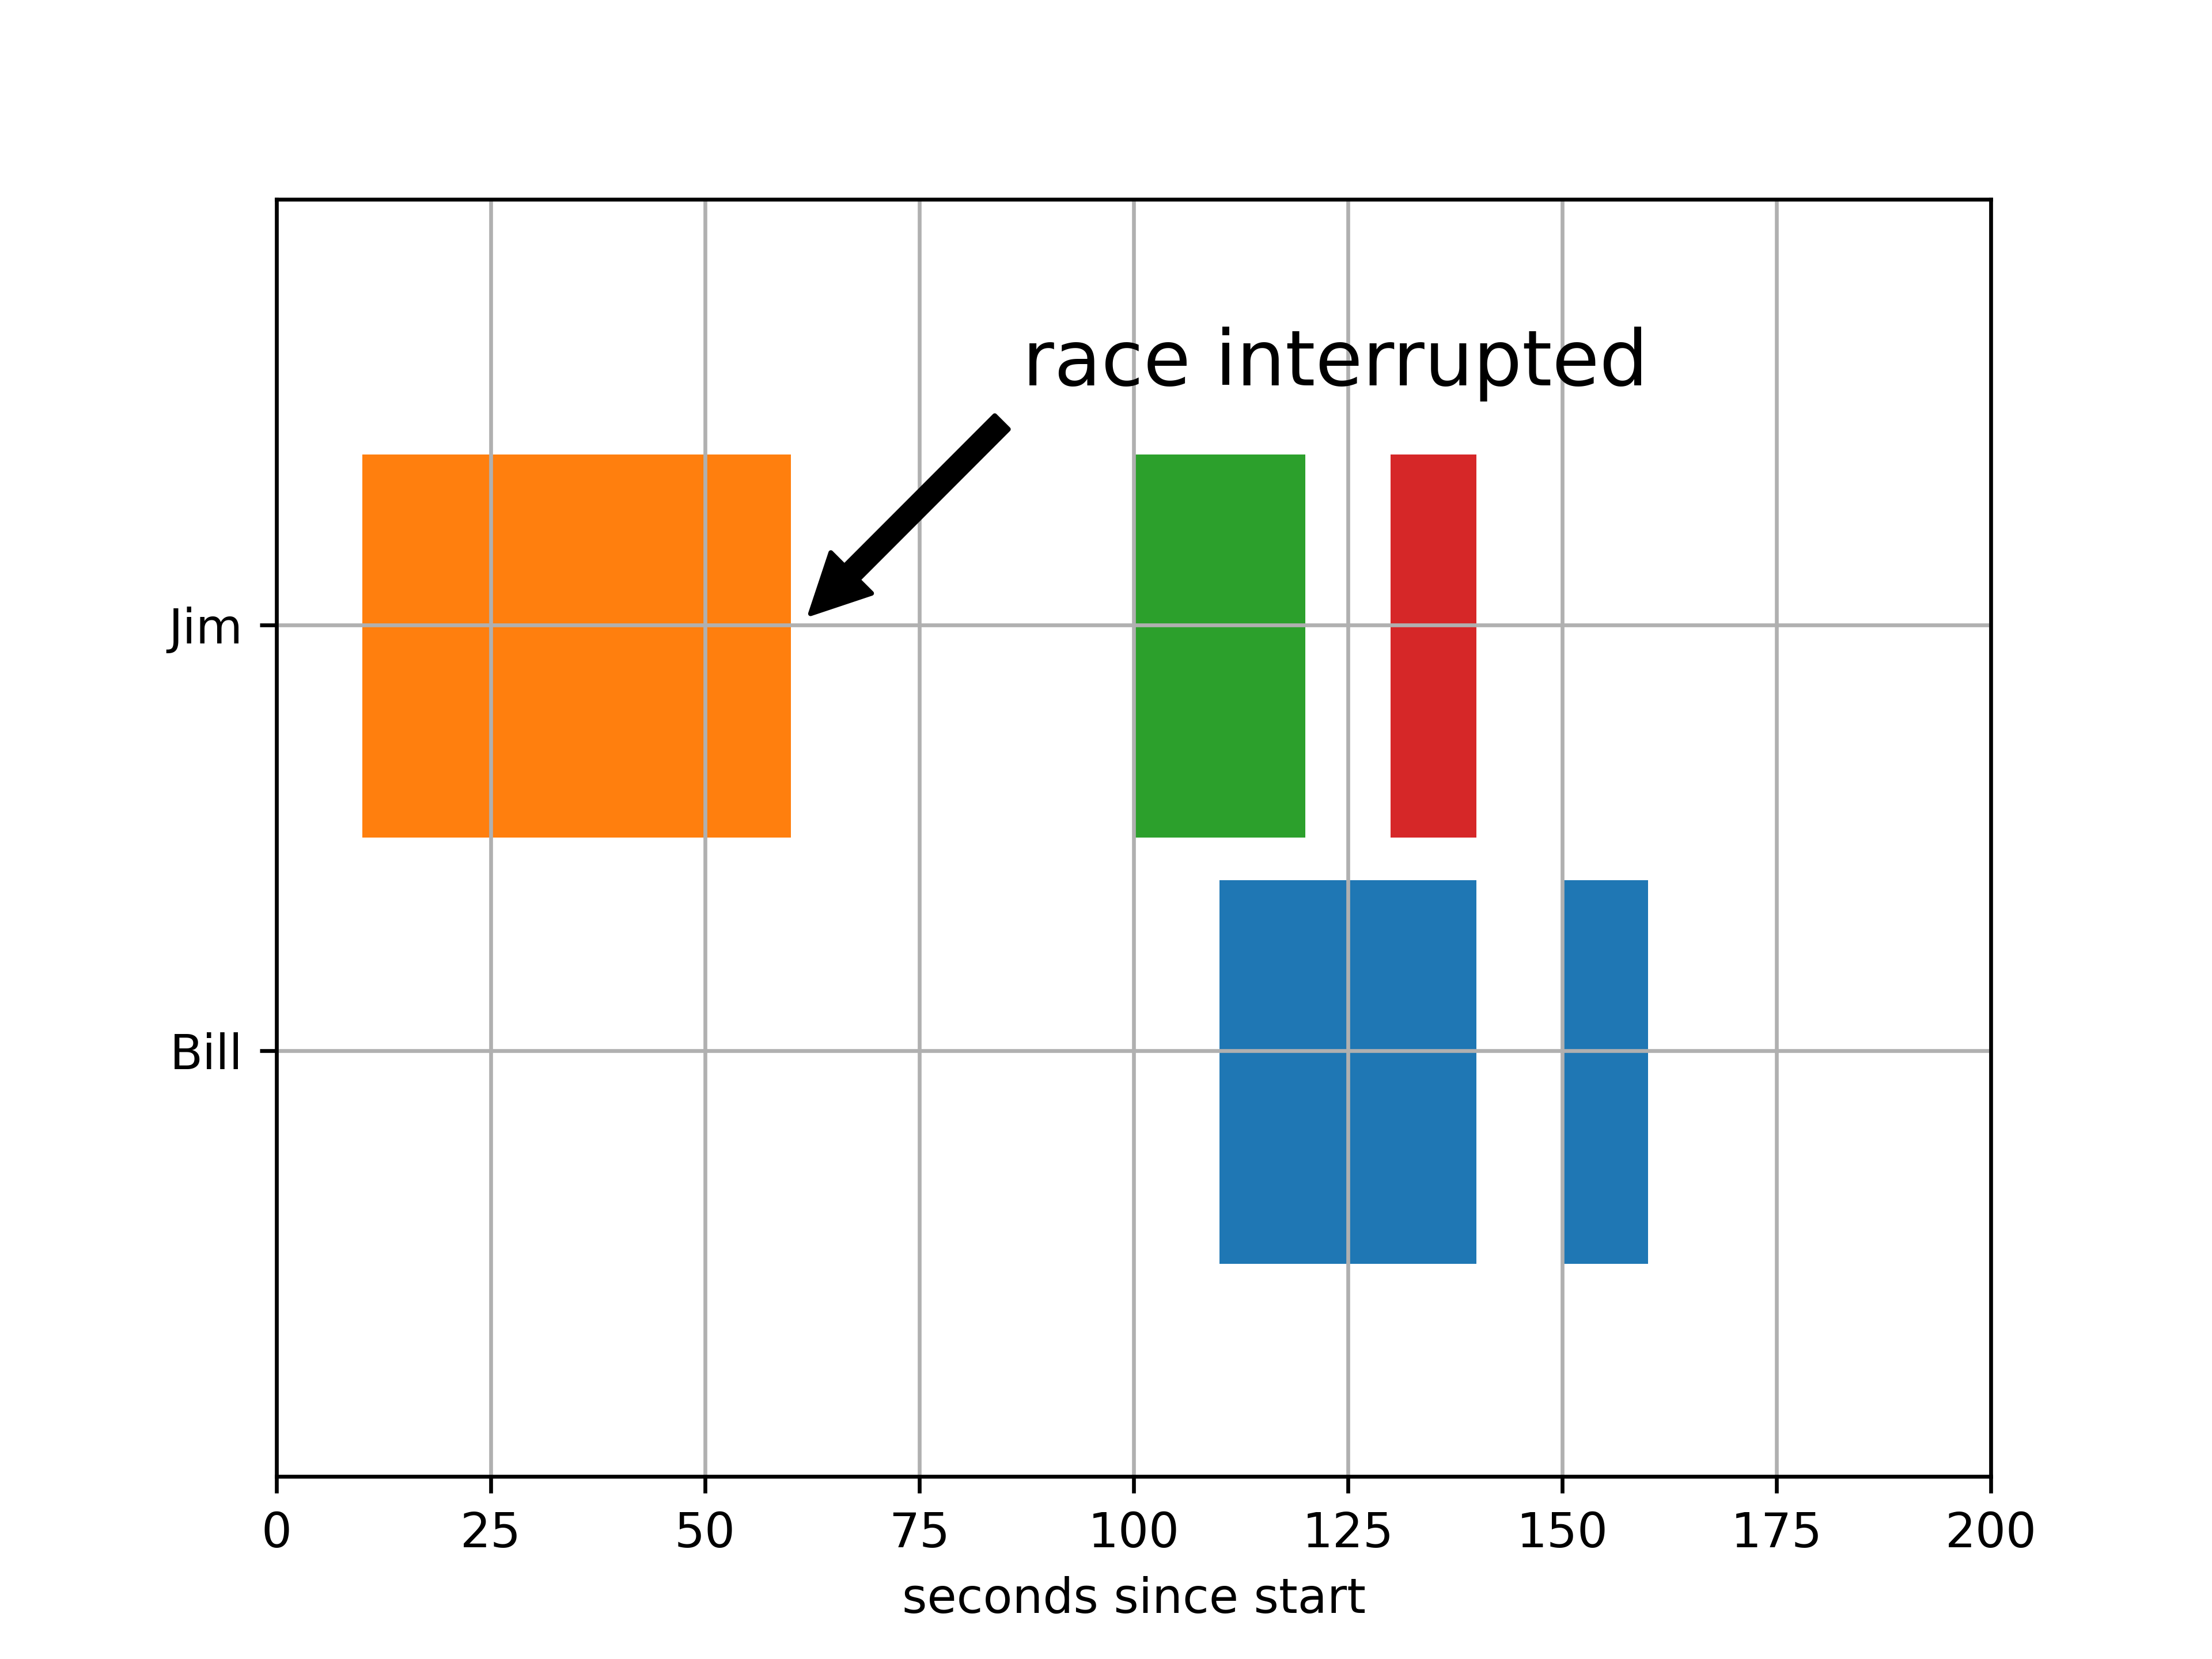
\includegraphics[width=0.6 \textwidth]{figs/chapter9/bars/BrokenBar}
\caption{破碎的条形图}
\end{figure}

\section{散点图}
\section{饼图}
\section{地图}
\section{热力图}
\section{表格}
\section{形象化描述}
\section{地图}
\section{热力图}
\chapter{数值参数}
\part{LATEX论文写作}

%% 附录
\appendix
\cleardoublepage


%% appendix chapter style
\titleformat{\chapter}[display]
{\bfseries}
{\flushright\zihao{4}附录\thechapter}
{1ex}
{
  \hrule width \hsize height .5pt
  \vspace{-2ex}\flushright\zihao{2}
}[\vspace{5ex}]


\chapter{Angular CLI}

\begin{lstlisting}[language=bash,style=shellstyle]
  ng new appname --style scss --skip-install
\end{lstlisting}


\backmatter


\cleardoublepage
%% 索引
\printindex

%% 参考文献
\bibliographystyle{plain}

\end{document}

%%% Local Variables:
%%% mode: latex
%%% TeX-master: t
%%% End:
